% MS-Thesis
\documentclass[11pt]{mvlthesis}
\usepackage[dvipdfmx]{graphicx}
\usepackage{verbatim,amssymb,amsmath,subfig,tabularx,ragged2e,booktabs}
\usepackage{float}
\usepackage{adjustbox}
\usepackage{placeins}
%\usepackage{wrapfig}
%\usepackage{lscape}
\usepackage{rotating}
\usepackage{graphicx}
\usepackage{cite}
\usepackage{url}
\usepackage[breaklinks = true]{hyperref}
\hypersetup{%
  colorlinks = true,
  linkcolor  = red
}
\usepackage{fancyvrb}
\usepackage[]{mcode}
%\usepackage{listings}
%%%%%%%%%%%%%%%%%%%%% SET UP ALL THE TITLE PAGE VARIABLES %%%%%%%%%%%%%%%%%%

\title{\scshape \mbox{Synthesizing Robust Training Data for}\\
\scshape \mbox{Machine Learning}}

\author{Kyle W. McClintick}
\thesis_or_diss{Thesis}
\degree_type{Master of Science}
\field{Electrical and Computer Engineering}
\degreeyear{December 2018}
\chair{Professor Alexander Wyglinski}
\chairtitle{Major Advisor}
\membertwo{x}
\memberthree{x}


%%%%%%%%%%%%%%%%%%%%%% INCLUDE USER DEFINED COMMANDS %%%%%%%%%%%%%%%%%%%%%%%
\newcolumntype{L}{>{\RaggedRight\arraybackslash}X}
\newcommand{\bi}{\begin{itemize}}
\newcommand{\ei}{\end{itemize}}
\newcommand{\ii}{\item}
\newcommand{\uvec}[1]{\boldsymbol{\hat{\textbf{#1}}}}
\newcommand{\be}{\begin{enumerate}}
\newcommand{\ee}{\end{enumerate}}
\newcommand{\ie}{\item}
\newcommand{\hv}{\mathbf{h}}
\newcommand{\Hmat}{\mathbf{H}}
\newcommand{\Emat}{\mathbf{E}}
\newcommand{\Dmat}{\mathbf{D}}
\newcommand{\ba}{\begin{align}}
\newcommand{\ea}{\end{align}}
\DeclareMathOperator\erf{erf}
\DeclareMathOperator*{\argmax}{arg\,max}

\newcommand{\fig}[5]{
    \begin{figure}[#1]
    \begin{center}
    \includegraphics[#2]{#3}
    \end{center}
    \caption{#4}
    \label{#5}
    \end{figure}
}
%%%%%%%%%%%%%% SPECIFY WHICH PARTS OF THE THESIS YOU WANT PRINTED %%%%%%%%%%

\renewcommand{\baselinestretch}{1.5}

\newcommand{\pderiv}[2]{\mbox{$\frac{\displaystyle \partial #1}{\displaystyle \partial #2}$}}

%%%%%%%%%%%%%%%%%%%% Done with setup, document starts here %%%%%%%%%%%%%%%%%
\begin{document}


%%%%%%%%%%%%%%%%%%%%%%%%%%%%%% TITLE + ABSTRACT %%%%%%%%%%%%%%%%%%%%%%%%%%%%
\maketitle
\begin{abstract}

Developing machine learning-based signal classifiers that generalize well requires training data that capture the underlying probability distribution of real signals. To synthesize a set of training data that can capture the large variance in signal characteristics, a robust, low bias, low decay framework that can support arbitrary baseband signals and channel conditions is required. Furthermore, domain adaptation can allow for powerful generalized training via transforms on unlabeled evaluation-time signals. Together, domain transforms and a robust training set can train a deep neural net to perform well in many real-world scenarios.

\end{abstract}

%%%%%%%%%%%%%%%%%%%%%% ACKNOWLEDGMENTS + TABLE OF CONTENTS %%%%%%%%%%%%%%%%%
\begin{frontmatter}
\begin{acknowledgements}
\begin{center}
\vspace{0.4in}
I would like to express my deepest gratitude to my advisor Professor Alexander Wyglinski for his continuous guidance and support towards my degree. I am very thankful for the opportunity to work with him in the Wireless Innovation Laboratory at Worcester Polytechnic Institute. 

I want to thank Professor Kaveh Pahlavan and Dr. Travis Collins for serving on my committee and providing valuable suggestions and comments with regards to my thesis. 

I would also like to thank my WILab team members Dr. Srikanth Pagadarai, Kuldeep, Renato, and Nivetha for their immense support during my graduate studies. I would like to thank my friends abroad and in the states who have stayed in contact and given me the support I need, including my friends from Audrey Ave: Alex and the Armstrongs, Ben, Elissa, Ivan, Thomas, and Vlad, my fraternity brothers from Lambda Chi Alpha and Theta Xi, who are too many to mention here, and the Lakeside bunch: Alia, Kelly, Gene, Jack, Jon, Nate, and Nic. I would like to thank good beer, catchy music, and sunny weekends. Finally, I'm thankful for my lovely girlfriend Zhijie, and my warm family: Colin, Dawn, and George. Without their constant support I wouldn't have finished this thesis.

\end{center}
\end{acknowledgements}

%\begin{frontmatter}
\tableofcontents
\listoffigures
\listoftables

\end{frontmatter}

%%%%%%%%%%%%%%%%%%%% INCLUDE THE REST OF THE DOCUMENT %%%%%%%%%%%%%%%%%%%%%%


%\chapter{Introduction}
\label{ch:introduction}
\section{Motivation}
what deep nets offer the communications world, why generalized training is needed to make deep nets perform well

\section{State of the Art}
current forms of communications generalized training

discuss rml

\section{Current Issues}
issues in generalized training...what happens when false assumptions made? perturbations?	

\section{Thesis Contributions}
This work contains the following contributions:
\begin{itemize}
\item A low decay, low bias framework is presented in Chapter~\ref{chapter3}, as well as example wave-forms and data sets that have low entropy.
\item Ongoing work on wireless channel domain adaptation in Chapter~\ref{chapter4}, including neural net architecture and initial results.
\end{itemize}

\section{Thesis Organization}
The thesis will be organized as follows: Chapter~\ref{chapter2} will give a survey of background knowledge learned by the author on the topics of wireless channel modeling (Section~\ref{chanmods}), neural networks with an emphasis on training and data sets (Section~\ref{training}), and modulation classification (Section~\ref{modclass}). Chapter~\ref{chapter3} presents the author's work on generalized training through the development and use of a low bias, low decay framework that synthesizes low-entropy data sets modeling state-of-the-art wave-forms. Finally, Chapter~\ref{chapter4} present's the author's ongoing work on generalized training through the use of the domain adaptation technique, and concluding thoughts are discussed in Chapter~\ref{conclusion}.

\section{List of Related Publications}
The following publications resulted from the activities of this thesis research:
\begin{itemize}
	\item K. McClintick, A. Wyglinski. “Physical Layer Neural Network Framework for Training Data Formation.” VTC Chicago, Fall 2018.
	\item K. Gill, K. McClintick, N. Kanthasamy, “Experimental Test-Bed for Bumblebee-Inspired Channel Selection in an Ad-hoc Network.” VTC Chicago, Fall 2018.
\end{itemize}
\chapter{Introduction}
\label{ch:introduction}
\section{Motivation}
what deep nets offer the communications world, why generalized training is needed to make deep nets perform well

\section{State of the Art}
current forms of communications generalized training

discuss rml

\section{Current Issues}
issues in generalized training...what happens when false assumptions made? perturbations?	

\section{Thesis Contributions}
This work contains the following contributions:
\begin{itemize}
\item A low decay, low bias framework is presented in Chapter~\ref{chapter3}, as well as example wave-forms and data sets that have low entropy.
\item Ongoing work on wireless channel domain adaptation in Chapter~\ref{chapter4}, including neural net architecture and initial results.
\end{itemize}

\section{Thesis Organization}
The thesis will be organized as follows: Chapter~\ref{chapter2} will give a survey of background knowledge learned by the author on the topics of wireless channel modeling (Section~\ref{chanmods}), neural networks with an emphasis on training and data sets (Section~\ref{training}), and modulation classification (Section~\ref{modclass}). Chapter~\ref{chapter3} presents the author's work on generalized training through the development and use of a low bias, low decay framework that synthesizes low-entropy data sets modeling state-of-the-art wave-forms. Finally, Chapter~\ref{chapter4} present's the author's ongoing work on generalized training through the use of the domain adaptation technique, and concluding thoughts are discussed in Chapter~\ref{conclusion}.

\section{List of Related Publications}
The following publications resulted from the activities of this thesis research:
\begin{itemize}
	\item K. McClintick, A. Wyglinski. “Physical Layer Neural Network Framework for Training Data Formation.” VTC Chicago, Fall 2018.
	\item K. Gill, K. McClintick, N. Kanthasamy, “Experimental Test-Bed for Bumblebee-Inspired Channel Selection in an Ad-hoc Network.” VTC Chicago, Fall 2018.
\end{itemize}

%% Heterogeneous CSS intro
\chapter{Data Synthesis and Neural Networks}
\label{chapter2}
The differences between physical layer ML and other ML domains are highlighted in~\cite{o2016radio}, drawing attention to the unique challenges the physical layer ML domain faces. Although transmitted wave-forms begin as well defined, man-made, synthetic structures, a virtually endless number of probabalistic, and sometimes non-linear, phenomenom alter the observed wave-forms receive-side. Even within a single phenomenom, there can exist again a virtually endless number of realizations or types of that imperfection. Some of the most prevelent and common imperfections include:
\begin{enumerate}
	\item Carrier Frequency Offset of both the transmitter and receiver's local oscillators, which drive each radio's mixers
	\item Phase Ambiguity introduced by the unknown distance between transmitter and receiver
	\item Random Symbol Timing Offset resulting from independently running sample clocks
	\item Additive White Gaussian Noise, bursty noise from phenomenom such as weather, interference from same and adjacent channels
	\item Wide-band phase rotation resulting in constructive and destructive phase wave-form copies created by reflectors
	\item Narrow-band Delay Spread due to multi-path interference
	\item Random signal arrival times due to MAC and Network layer architectures and schedules
	\item Doppler Shifts resulting from motion of the transmitter, receiver, or scatterers and reflectors within the wireless channel
\end{enumerate}

\section{The Radio Frequency Front End}
tx rx chain, complications, ways to correct

\section{Classical Channel Models}
list the modeling algorithms

\section{Machine Learning Algorithms}
loss functions, etc

\section{Neural Network Architectures}
layers, roles, types, etc


\section{Summary}
review and conclude\\


%% LTE-R analysis intro
\chapter{Physical Layer Neural Network Framework for Training Data Formation}
\label{chapter3}

We present a novel open-source dataset modification framework designed to study the effect of wireless channels on the training and testing of modulation classifiers employing Neural Networks (NN). Communication systems optimize for capacity by packing information bits very closely together. Consequently, RF datasets contain less redundancy and context than other NN domains such as image and speech classification. As a result, NN performance is poor when brought to implementation if training is not done with datasets properly describing gathered test sets. Our framework pushes datasets through a sequential, parallelized, modular, block-style set of wireless channels, where blocks can be written by operators or pulled from a core library. Utilizing our datasets, we perform analysis of a NN. We determine the NN requires datasets collected by a receiver capable of phase correction to below 4 degrees offset, and Carrier Frequency Offset (CFO) correction to below $\bf{1\%}$ normalized to sample rate to maintain near-peak modulation classification accuracy.

\subsection{Introduction}
\label{sec1}

There exist numerous approaches published in open literature to model wireless channels~\cite{tsb88tia}. Receive chains apply an equally numerous variation of corrections to signals to remove or limit channel effects on data through frame synchronization, CFO correction, timing corrections, and other methods~\cite{rappaport1996wireless}. Contributions to the field are met with scrutiny due to the maturity of these models and correction systems. However, NNs can adjust for nonlinearities unaccounted for by classical communication and information theory\cite{schenk2008rf}. Significant gains can be achieved by breaking the traditionally sequential nature of activities performed by transmit and receive chains~\cite{wymeersch2007iterative}. Additionally, recent NN publications have shown high-capacity learning algorithms that have demonstrated high energy efficiency and computational throughput~\cite{raina2009large}. Consequentially, interest has been expressed~\cite{8054694, wang2017deep} for the use of NNs in physical layer communications. NN applications in the physical layer can be classified into two categories: end-to-end autoencoders that determine unknown hidden layers to recreate an input data layer at an output data layer, and NNs that determine specific design choices of the physical layer.

For any physical layer NN, an often used framework for dataset generation is GNU Radio Companion's (GRC) channel model blocks. Each channel block offers a modular, sequential, parallelized method of dataset manipulation. While a powerful tool, GRCs gpl3 license makes privacy of work difficult for companies with export control and Non-Disclosure Agreements (NDA). Most all blocks must be written by the user which require documentation, upkeep, and time. Additionally, GRC is better at some use cases than others, requiring creativity to generate some datasets. Most importantly, GRC cannot easily and properly construct massive arrays of varied wireless channels.

In~\cite{o2016radio}, a dataset is generated for use in a NN modulation classifier, and interest is expressed for "iteratively better, more complex, and more challenging datasets", which "will be required to help compare, measure, and evaluate these (communication) tasks". It is the fundamental assumption made in supervised learning of a NN that the training data is representative of practical data. That assumption cannot be broken in data partitioning or through a lack of resolution in the distribution of training data. For many NNs, that assumption is broken by the highly unique nature of wireless transmissions, which are varied by a virtually endless number of channel effects.

In this paper, we propose a framework that creates datasets satisfying this assumption through their size and diversity in a computationally efficient, parallelized method. Channel effects are sequentially applied to complex valued datasets in a modular way, where channel blocks are chosen by a configuration file from a library or user created blocks. Channels described by design parameters can be iterated through, achieving thorough file multiplication labeled in a clear and concise way.

This paper presents our framework in section~\ref{sec2}, and discusses implementation details of training and testing in section~\ref{sec3}. Section~\ref{sec4} displays simulation results, and concluding thoughts are presented in section ~\ref{sec5}.

\subsection{Proposed Framework}
\label{sec2}

\begin{figure*}[ht!]
	\centering	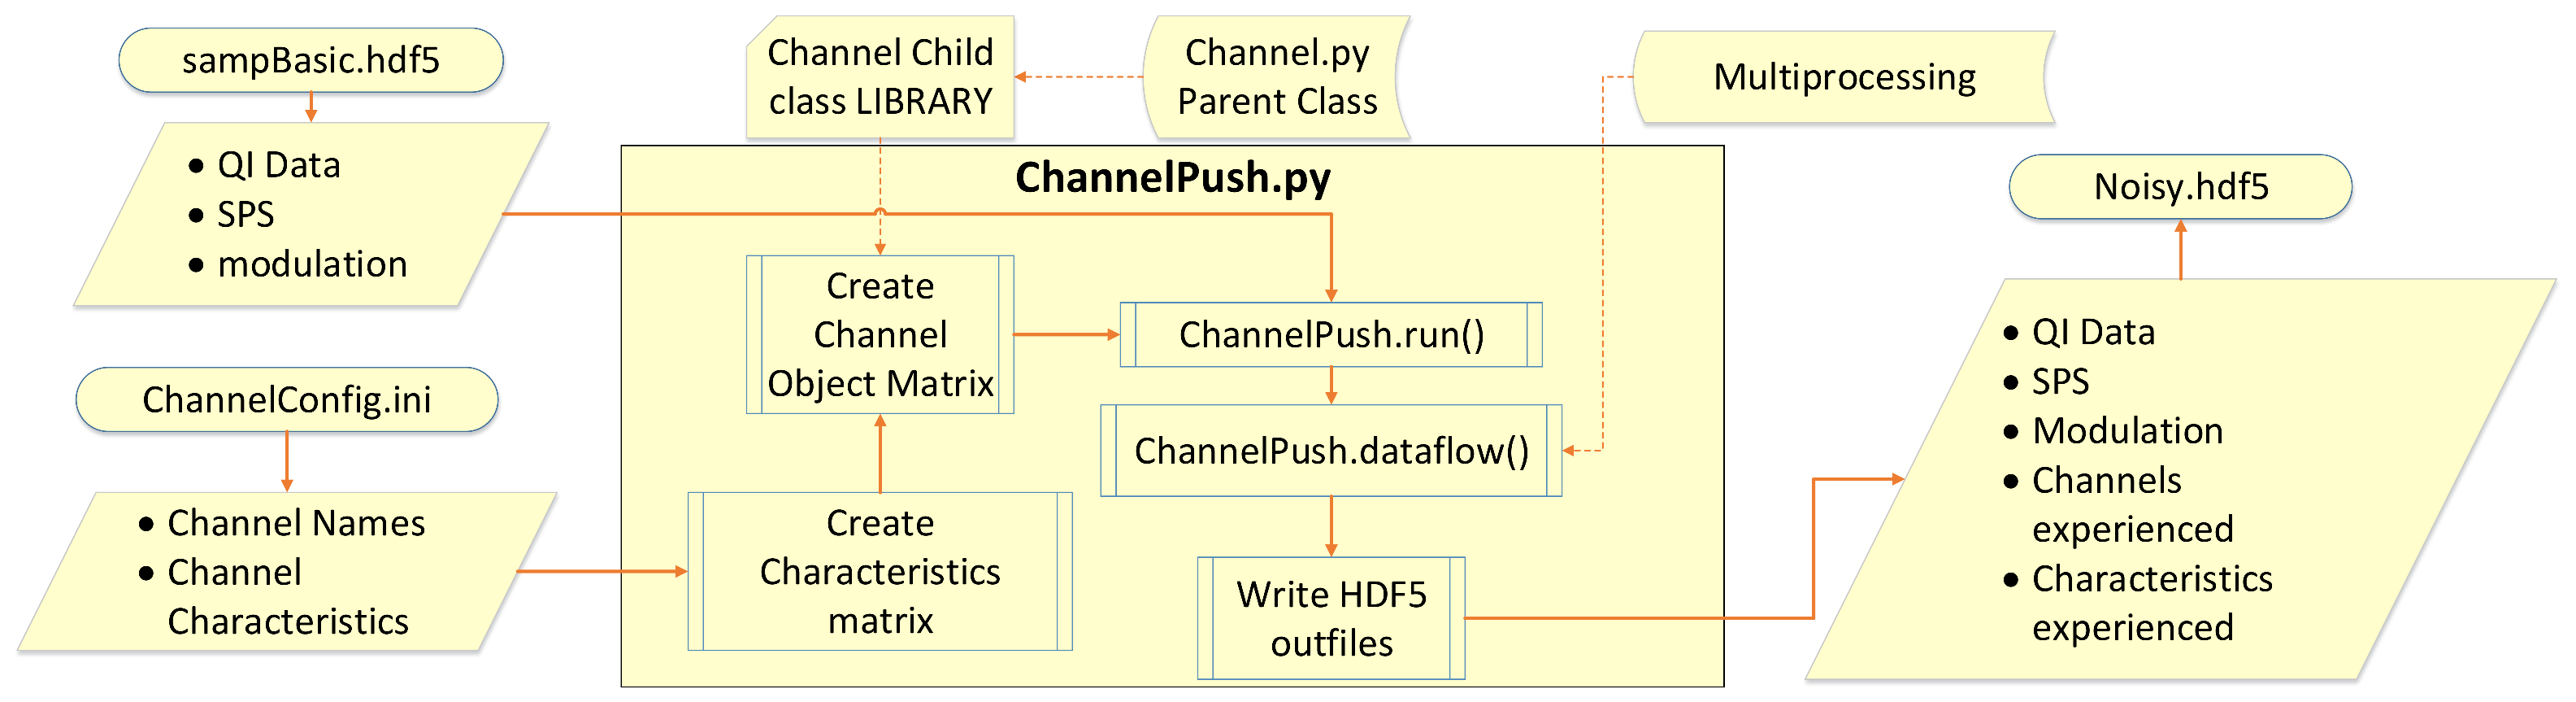
\includegraphics[width=1\textwidth,keepaspectratio]{figs/channelpush_paper.eps}
    \caption{ChannelPush.py takes in sampBasic.hdf5 and ChannelConfig.ini as inputs, and writes one or many Noisey.hdf5 outfiles. In the create channel object matrix sub-process, the channel library is used to initialize channel objects, which inherit from the channel parent class. The dataflow() function sequentially pushes data through each list of channels in parallel, making use of the Multiprocessing package.} 
\label{fig:channeltoolsub}      
\end{figure*}

Section~\ref{sec4} of this paper and \cite{8170853} display a clear need to consider the radio front end and wireless channel effects in any NN experiment. NNs must either be trained with datasets effected by channel effects or tested with datasets gathered by receivers that correct for channel effects to maintain near-peak accuracy. Either condition must be met to maintain the fundamental training assumption by expanding training datasets to represent test datasets, or to bound test datasets to represent training datasets. The latter is often preferable, as more complex training datasets always yield lower peak accuracy. Our framework generates supersets of data that can be used to help make this training decision, and to what extent training complexity should be taken for different wireless channel phenomenon. By testing NNs with supersets from our framework, certain physical layer corrections may be revealed to be unnecessary, inadequate, or overly-complex. As an example, a NN experiment makes use of a frame synchronization block created by the user to create a superset from their Dataset Under Test (DUT). A resulting conclusion on their NNs performance might be that a longer Barker Code must be used, reducing data throughput, or training must be done with a greater range of frame synchronization errors, reducing peak NN performance. This might not be an easy decision, requiring multiple uses of our framework to hypothesize, train, and evaluate NN performance and data throughput.

The inputs and outputs of the framework are described in Figure~\ref{fig:channeltoolsub}. The framework requires a DUT and instructions for which channel blocks to push the DUT through. Framework outputs are instances of the DUT that have been modified by a unique combination of channel block realizations. Any type or amount of channel blocks may be used from a library by editing the instructions. The DUT is pushed through channel blocks one sample at a time. Channel objects may be added, modified, or removed from the framework by minimal editing of the instructions. Each output is computed and written in a separate Central Processing Unit (CPU) process.

To experiment with supersets created with our framework, training and testing is done in~\cite{convnetmodrec} with Keras2, an Application programming interface (API). TensorFlow, an open-source software library that makes use of data flow graphs to perform numerical computations, is used as the backend. In our training and testing, the DUT is divided into training and testing sets, making sure there is no overlap of values. We utilize a sequential NN, which is composed of layers which only interact with their neighboring layers. Common sequential NN layers include reshape, zeropadding2D, convolutional2D, dropout, flatten, activation, and dense layers. Reshape layers adjust the height and width of layer nodes structures and batch size (which determine the number of training parameters). Zeropadding2D adds zero values to node's sides, tops, and bottoms. Convolutional2D inputs are convolved over 2 dimensions to produce a tensor of outputs functioning as hidden layers between input and output layers. Dropout layers randomly set a fraction of the inputs to 0 at each update during training to prevent overfitting. Flatten layers reduce the dimension of the input, often to reduce the last hidden layer's output shape to the smaller output layer's input shape. The activation and dense layers apply a non-linear function to inputs, most popularly a Mean Square Error (MSE) function.

Perhaps the most notable layer here is the activation layer, which applies a non-linear function to the layers inputs. During the most popular method of training, Stochastic Gradient Descent (SGD), training parameters are determined by an algorithm involving a loss function approximation. That approximation is described as a batch-normalized sum of non-linear functions. For an overview of Machine Learning (ML), the reader is directed towards section II of~\cite{8054694}

\subsection{Implementation}
\label{sec3}
In development, sampBasic.hdf5 has served as our DUT, a dataset of complex values representing constellation points of equiprobable random binary bits. In the hdf5 format, data can be assigned to subsets, and each subset, or the whole hdf5 file, assigned labels in the form of ['Key'] = value. Labels utilized are the Samples Per Symbol (SPS) or oversampling factor of the data, the source file of the dataset, the version of hdf5 the file is source encoded with, and the modulation type of the dataset. ChannelConfig.ini represents the configuration for the framework used in development. The .ini format follows a key = value format, organized under headers [HEADER], where all values are strings. Channels are described by keys 'channelx' under the [CHANNELS] header and 'characteristicsx' under the [CHARACTERISTICS] header. Each channel's characteristic parameters are '|' separated, while a sweep over that parameter's values are comma separated. Each channel realization writes a uniquely modified version of the DUT as noiseyx.hdf5. This file multiplication can extend over any number of sequential channel objects, as seen in Figure~\ref{fig:channeltoolstructure}. Each output file utilizes hdf5's labeling capabilities, detailing the types of channels and parameter values of those channels that each file was pushed through in the form ['channel:parameter'] = value.

After the configuration file is imported, delimiters convert the configuration into a 3D matrix. Within this structure, each primary index signals a channel block type, the second a parameter, and the tertiary index a value of that parameter.

\begin{figure}[ht!]
	\centering	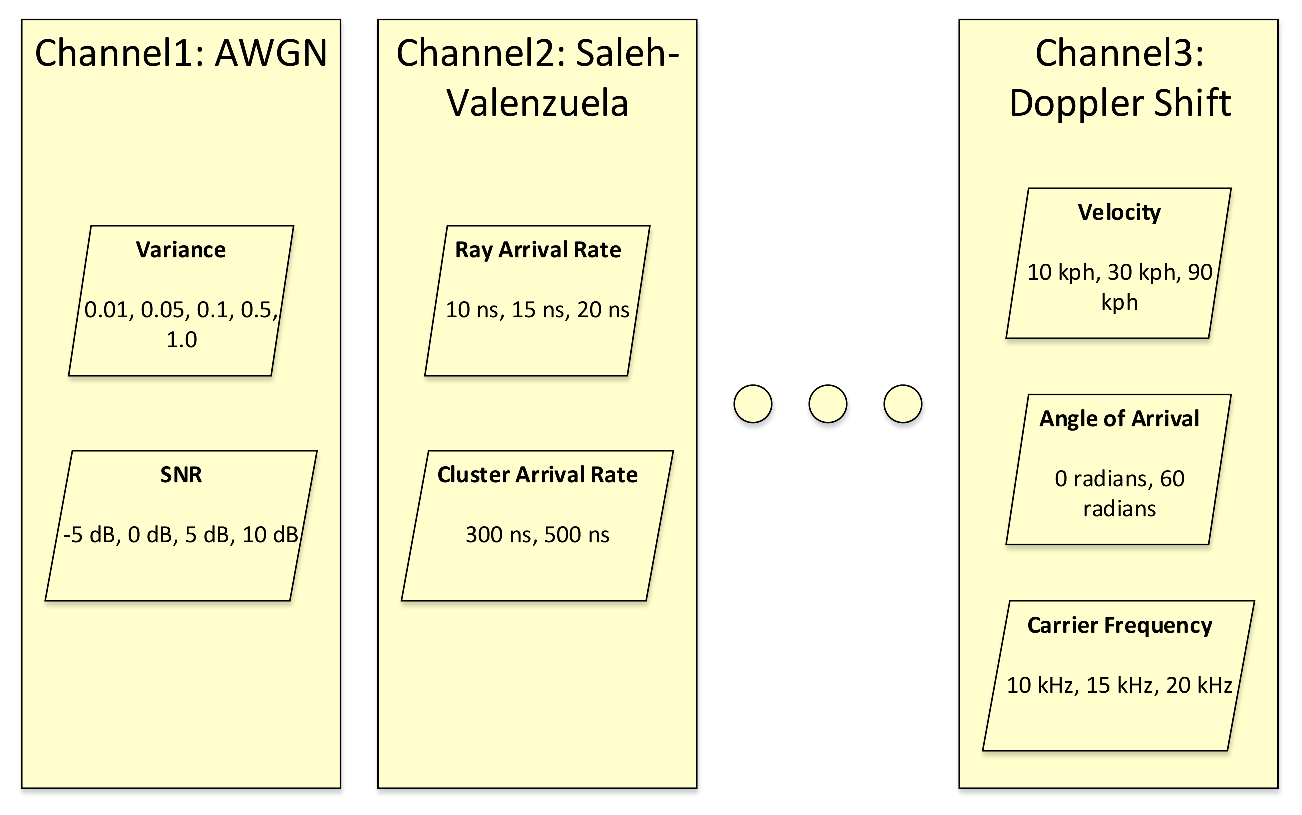
\includegraphics[width=0.45\textwidth,keepaspectratio]{figs/vtc_list_structure.eps}
    \caption{Example 2D channel matrix built from ChannelConfig.ini. There exist 20 AWGN, 6 Saleh-Valenzuela, and 18 Doppler Shift channel objects in this example, which will result in 2160 hdf5 files written. Each dataset features a unique combination of the 3 wireless channels modifying the same input dataset, with labels describing which realization was experienced} 
\label{fig:channeltoolstructure}      
\end{figure}

From that 3D matrix, a 2D matrix of channel objects is initialized, where the primary list signals grouping of channel types, and the secondary list is each realization of that channel type. Channel classes share similarities in the way they handle states, inputs, and outputs, so they inherit from a parent Channel class. A template exists to add a child channel class to the core library. in the run() function, the 2D matrix is fragmented into 1D lists of channel objects, where the total set of lists represents every possible sequential combination of unique channel realizations such that there is at least one of each channel type in each list. The next function call, dataflow(), sequentially modifies the input data by each channel of each list. This task, as well as file writing and attaching labels, is performed in parallel using the Multiprocessing import.

We modify~\cite{convnetmodrec} to run with a python3.5 interpreter instead of 2.7, using TensorFlow as a backend instead of Theano, as in the journal. The NN structure used is identical to theirs besides the dimensions of our datasets (see Table~\ref{table:tab1}). The dimension size change is due to a difference in Samples Per Symbol (SPS). The input layer has an output shape of (None, 1, 2, 4), having 4 channels as opposed to 128. This represents 4 samples of each symbol in our datasets rather than 128, where the data transmitted remains constant but probabilistic channel effects vary.

\begin{table*}[t!]
\centering
\caption{The structure of the NN used in section~\ref{sec4}. Each row represents a layer, where output shape is displayed as (batch, height, width, channels) and (batch\_size, input\_dim). Each layer is connected to the previous layer, and number of params is proportional to SPS and the size of convolutional layers.}
\begin{tabular}{c  c  c  c }
\toprule
Layer (type) & Output Shape & Param & Connected to\\\hline\hline
reshape\_1 (Reshape) & (None, 1, 2, 4) & 0 & reshape\_input\_1[0][0]\\
zeropadding2d\_1 (ZeroPadding2D) & (None, 1, 2, 8)    & 0       &    reshape\_1[0][0]\\
conv1 (Convolution2D)          &  (None, 256, 2, 6)  & 1024     &   zeropadding2d\_1[0][0]\\            
dropout\_1 (Dropout)            &  (None, 256, 2, 6)  & 0         &  conv1[0][0]\\
zeropadding2d\_2 (ZeroPadding2D) & (None, 256, 2, 10)  & 0          & dropout\_1[0][0]\\                 
conv2 (Convolution2D)          &  (None, 80, 1, 8)   & 122960     & zeropadding2d\_2[0][0]\\          
dropout\_2 (Dropout)           &   (None, 80, 1, 8)  &  0          & conv2[0][0]\\                  
flatten\_1 (Flatten)           &   (None, 640)      &   0          & dropout\_2[0][0]\\                 
dense1 (Dense)               &    (None, 256)       &    164096    & flatten\_1[0][0]\\                
dropout\_3 (Dropout)          &    (None, 256)      &     0          & dense1[0][0]\\                  
dense2 (Dense)               &    (None, 11)      &      2827       & dropout\_3[0][0]\\              
activation\_1 (Activation)   &     (None, 11)     &       0          & dense2[0][0]\\                 
reshape\_2 (Reshape)        &      (None, 11)    &        0    &       activation\_1[0][0]\\\hline\hline
Total params\: 290,907\\
Trainable params\: 290,907\\
Non-trainable params\: 0\\
\hline
\bottomrule
\end{tabular}
\label{table:tab1}
\end{table*}

\subsection{Simulation and Results}
\label{sec4}

In this paper, we focus on the wireless channel effect of CFO and phase ambiguity due to their computational simplicity. In any communication system, the transmitter and receiver typically are not using the same Local Oscillator (LO). This leads to issues in the baseband when a received signal is demodulated from its carrier frequency, proportional to the max possible frequency offset:

\begin{equation}
\label{eq3}
f_o,_{max} = \frac{f_c \times PPM}{10^6}
\end{equation}

\noindent where PPM is the maximum possible Parts Per Million offset of the LO, and $f_c$ is the received signal carrier frequency. We investigate the performance of~\cite{o2016convolutional} when the 2016.10a dataset has the additional channel effect of CFO, uncorrected by classical Coarse Frequency Correction (CFC) and Fine Frequency Correction (FFC) methods. As shown in~\cite{8170853}, testing done against channel effects not trained with causes classification accuracy to significantly decrease. We have observed a relationship between the complexity of the environment a NN is trained for and peak accuracy. Consequently, it should be the goal of any additional complexity in NN physical layer datasets to represent expected channel effects realistically. To obtain a realistic PDF of CFOs for training, ideally an infinite number of random values would maximize accuracy. However, training is very computationally expensive, so such a goal is unrealizable, particularly when the proposed framework is considered (as each additional channel type can represent one, or several, orders magnitude additional samples). Considering this, the datasets in Table~\ref{table:tab2} are presented to learn more about practical performance of the classifier~\cite{o2016convolutional}.

\begin{table}[ht!]
\centering
\caption{Four datasets generated with our framework. Datasets are trained, partitioned, and tested against a modulation classifier.}
\begin{tabular*}{0.5\textwidth}{c l c }
\toprule
Dataset & Description\\\hline
RML\_4sps & RML2016.10a dataset at 4 SPS and 0 CFO\\
CFO\_grc & RML\_4sps trained with GRC's dynamic channel\\
CFO\_super & RML\_4sps file multiplied over 100 discrete CFOs channels\\
 & evenly spaced from 0 to 20\% normalized to sample rate\\
Phase\_super & RML\_4sps file multiplied over 100 phase ambiguities evenly\\
 & spaced from 0 to $2\pi$ radians\\
\bottomrule
\end{tabular*}
\label{table:tab2}
\end{table}

The RML2016.10a dataset contains 1000 symbols, oversampled by a factor of 128, passed through GRC's dynamic channel model object, which has an 8-tap multipath profile of K-factor 4, fixed Doppler shift 1 Hz, random STO of variance 0.01 max value 50 samples, and random CFO of variance 0.01 max value $0.25\%$ normalized to 200 kHz sample rate. The dataset contains 11 modulation schemes (8 digital, 3 analog). SNR is swept from -20 dB to 20 dB in 2 dB steps. The CFO alter each sample of each dataset with the following phase rotation per sample:

\begin{equation}
\label{eq1}
\Theta[i] = e^{j\frac{0.2\times i}{N}\frac{2\pi}{sps}}
\end{equation}

\noindent where $N$ is the number of CFO values, $i = 0, 1...N-1$, and $sps$ is the oversampling factor. Since frequency is known as phase over time, the phase rotation at sample $k$ in a dataset for constant SNR, modulation type, and phase rotation per sample can be written as:

\begin{equation}
\label{eq4}
\phi[k, i] = \Theta[i]^k,~k=1,2...M
\end{equation}

\noindent where $M$ is the number of samples in a transmission with the above mentioned constants, and $\phi$ is only a function of $i$ for the phenomenon of initial phase offset. The CFO\_super test set aims to provide complete coverage of all possible CFO outcomes, making testing more reproducible and consistent. In Figure~\ref{fig:nocfo}, we present the accuracy of~\cite{o2016convolutional} in classifying the modulation scheme of data trained by RML\_4sps and tested by CFO\_super, data trained by CFO\_grc in Figure~\ref{fig:cfo}, and data trained by RML\_4sps and tested by Phase\_super in Figure~\ref{fig:phase}.

\begin{figure}[ht!]
	\centering	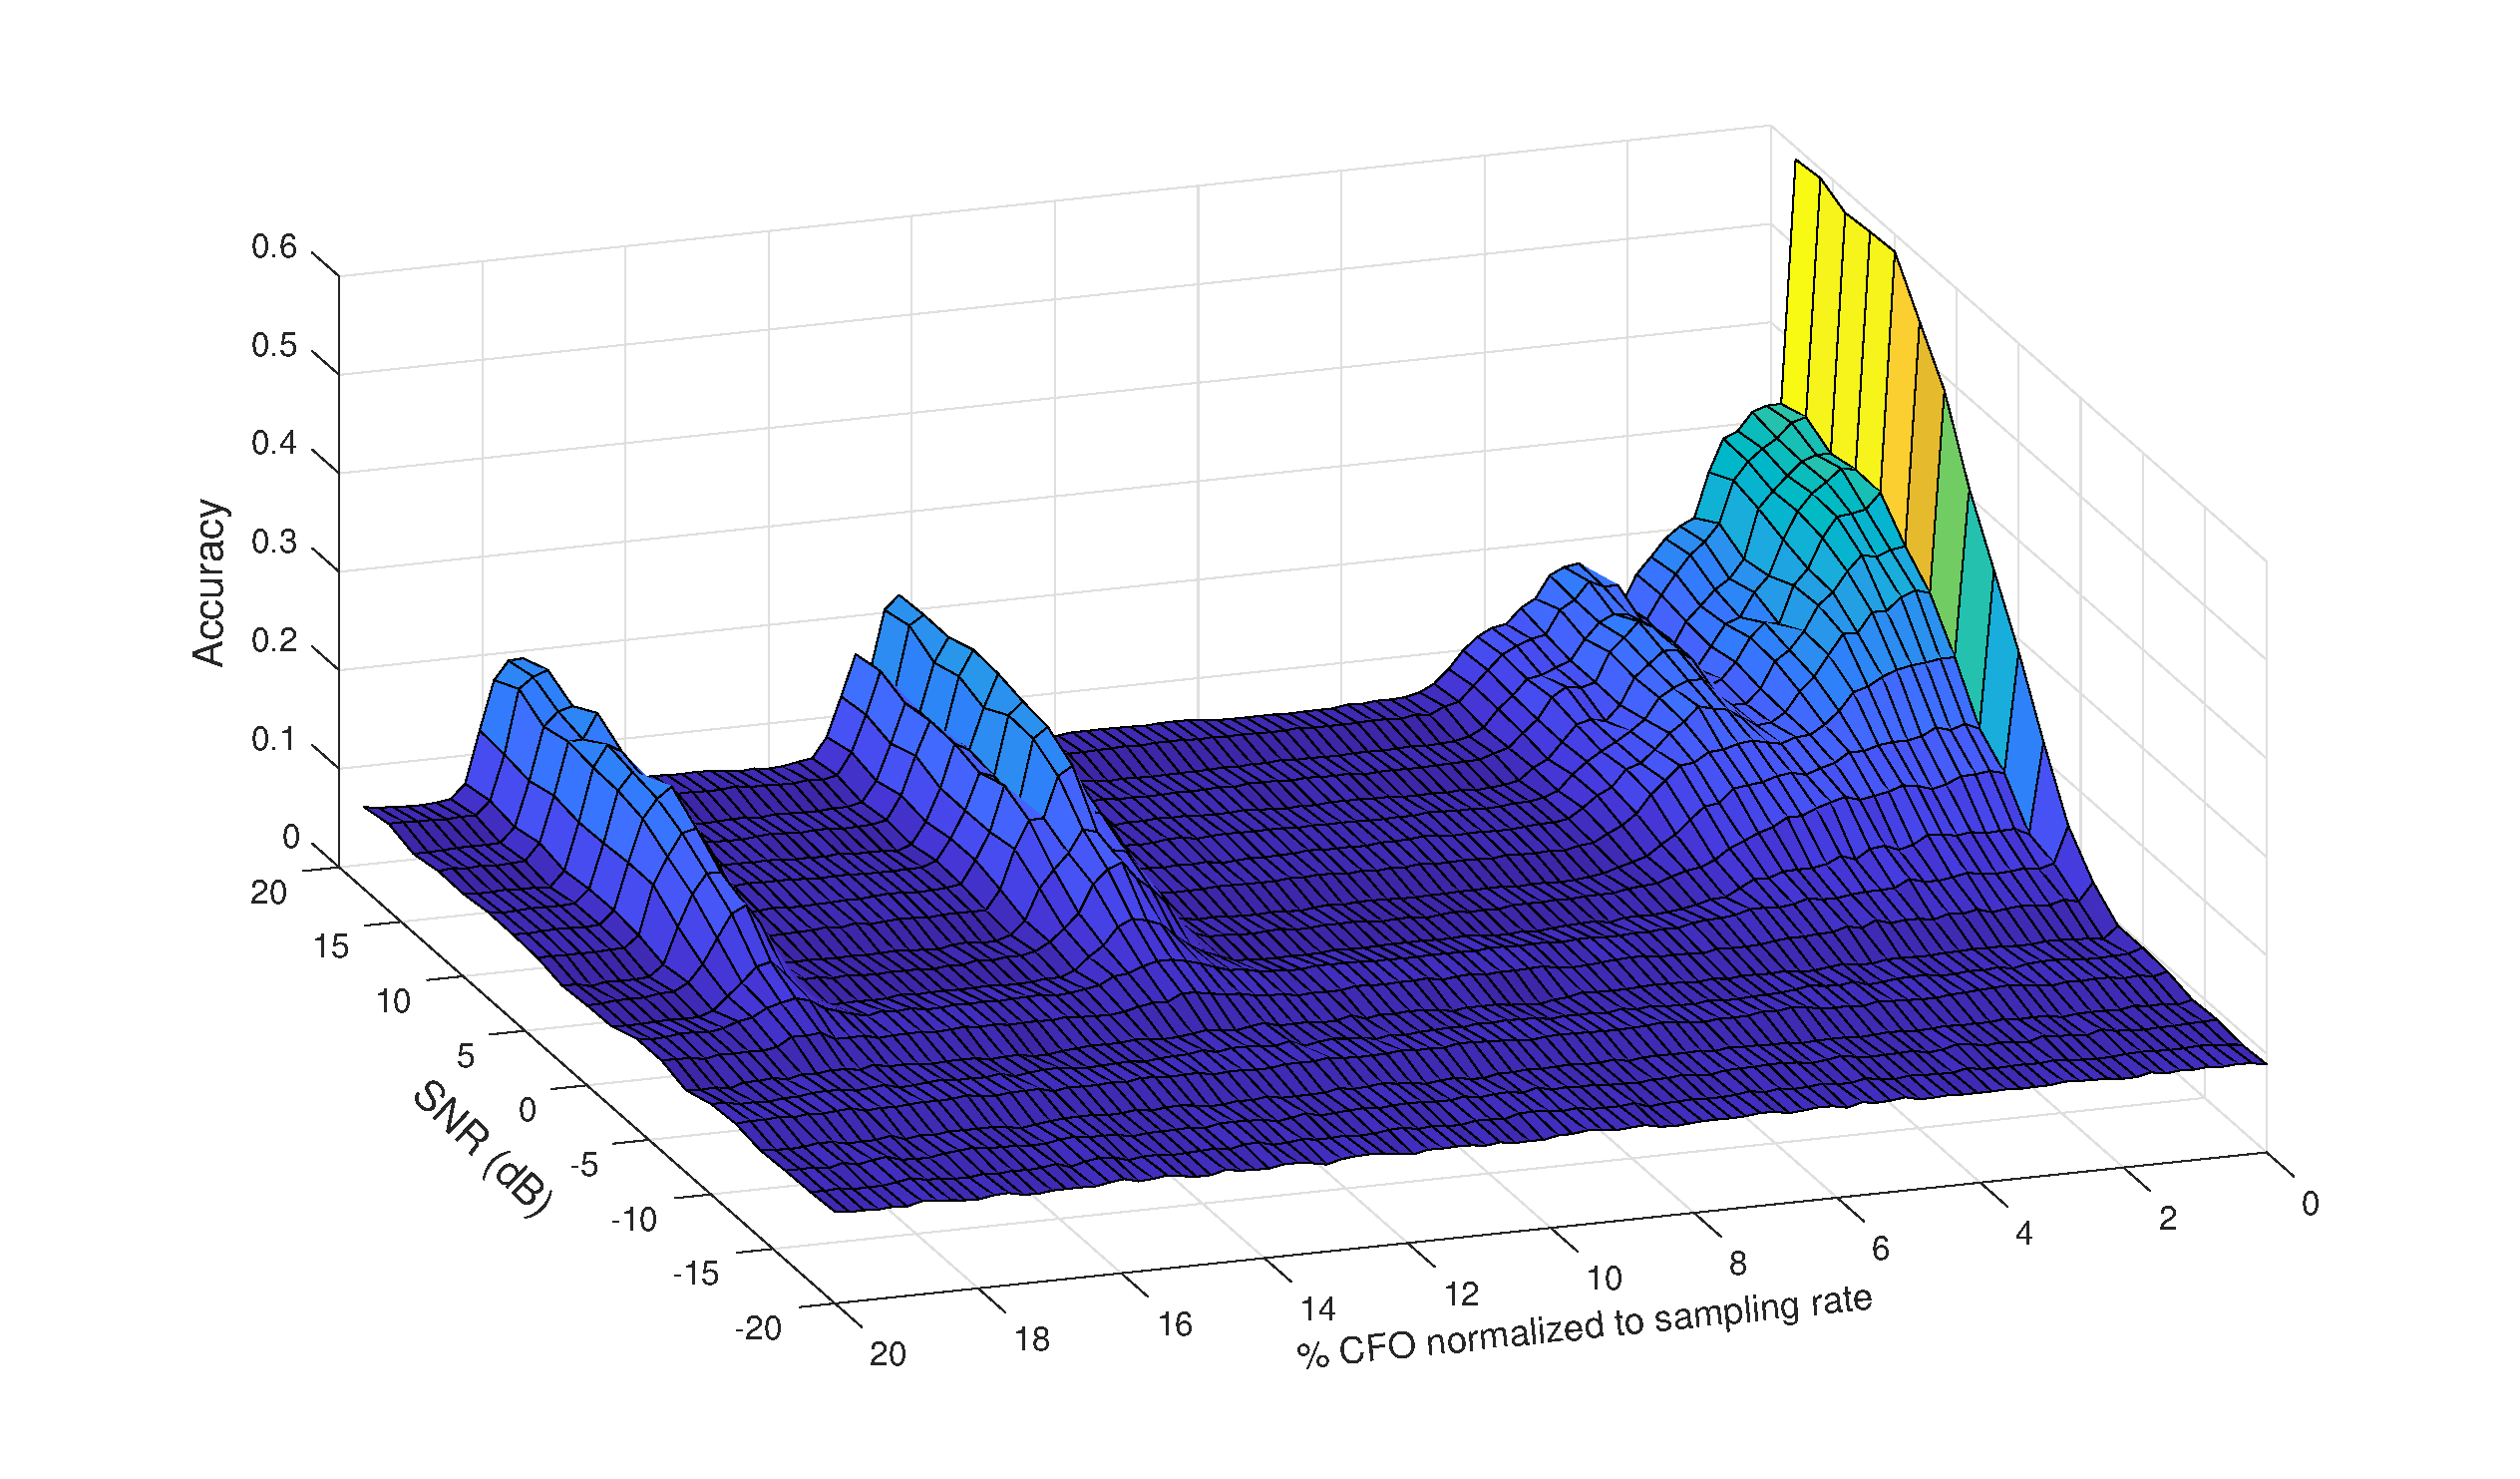
\includegraphics[width=0.45\textwidth,keepaspectratio]{figs/rml2016_nocfo.eps}
    \caption{CFO\_super test results when trained with RML\_4sps. Accuracy is averaged over 11 modulation schemes, and significantly decreases when tested against a CFO channel of just $0.2\%$ normalized to sample rate. Accuracy peaks at $60\%$.} 
\label{fig:nocfo}      
\end{figure}

\begin{figure}[ht!]
	\centering	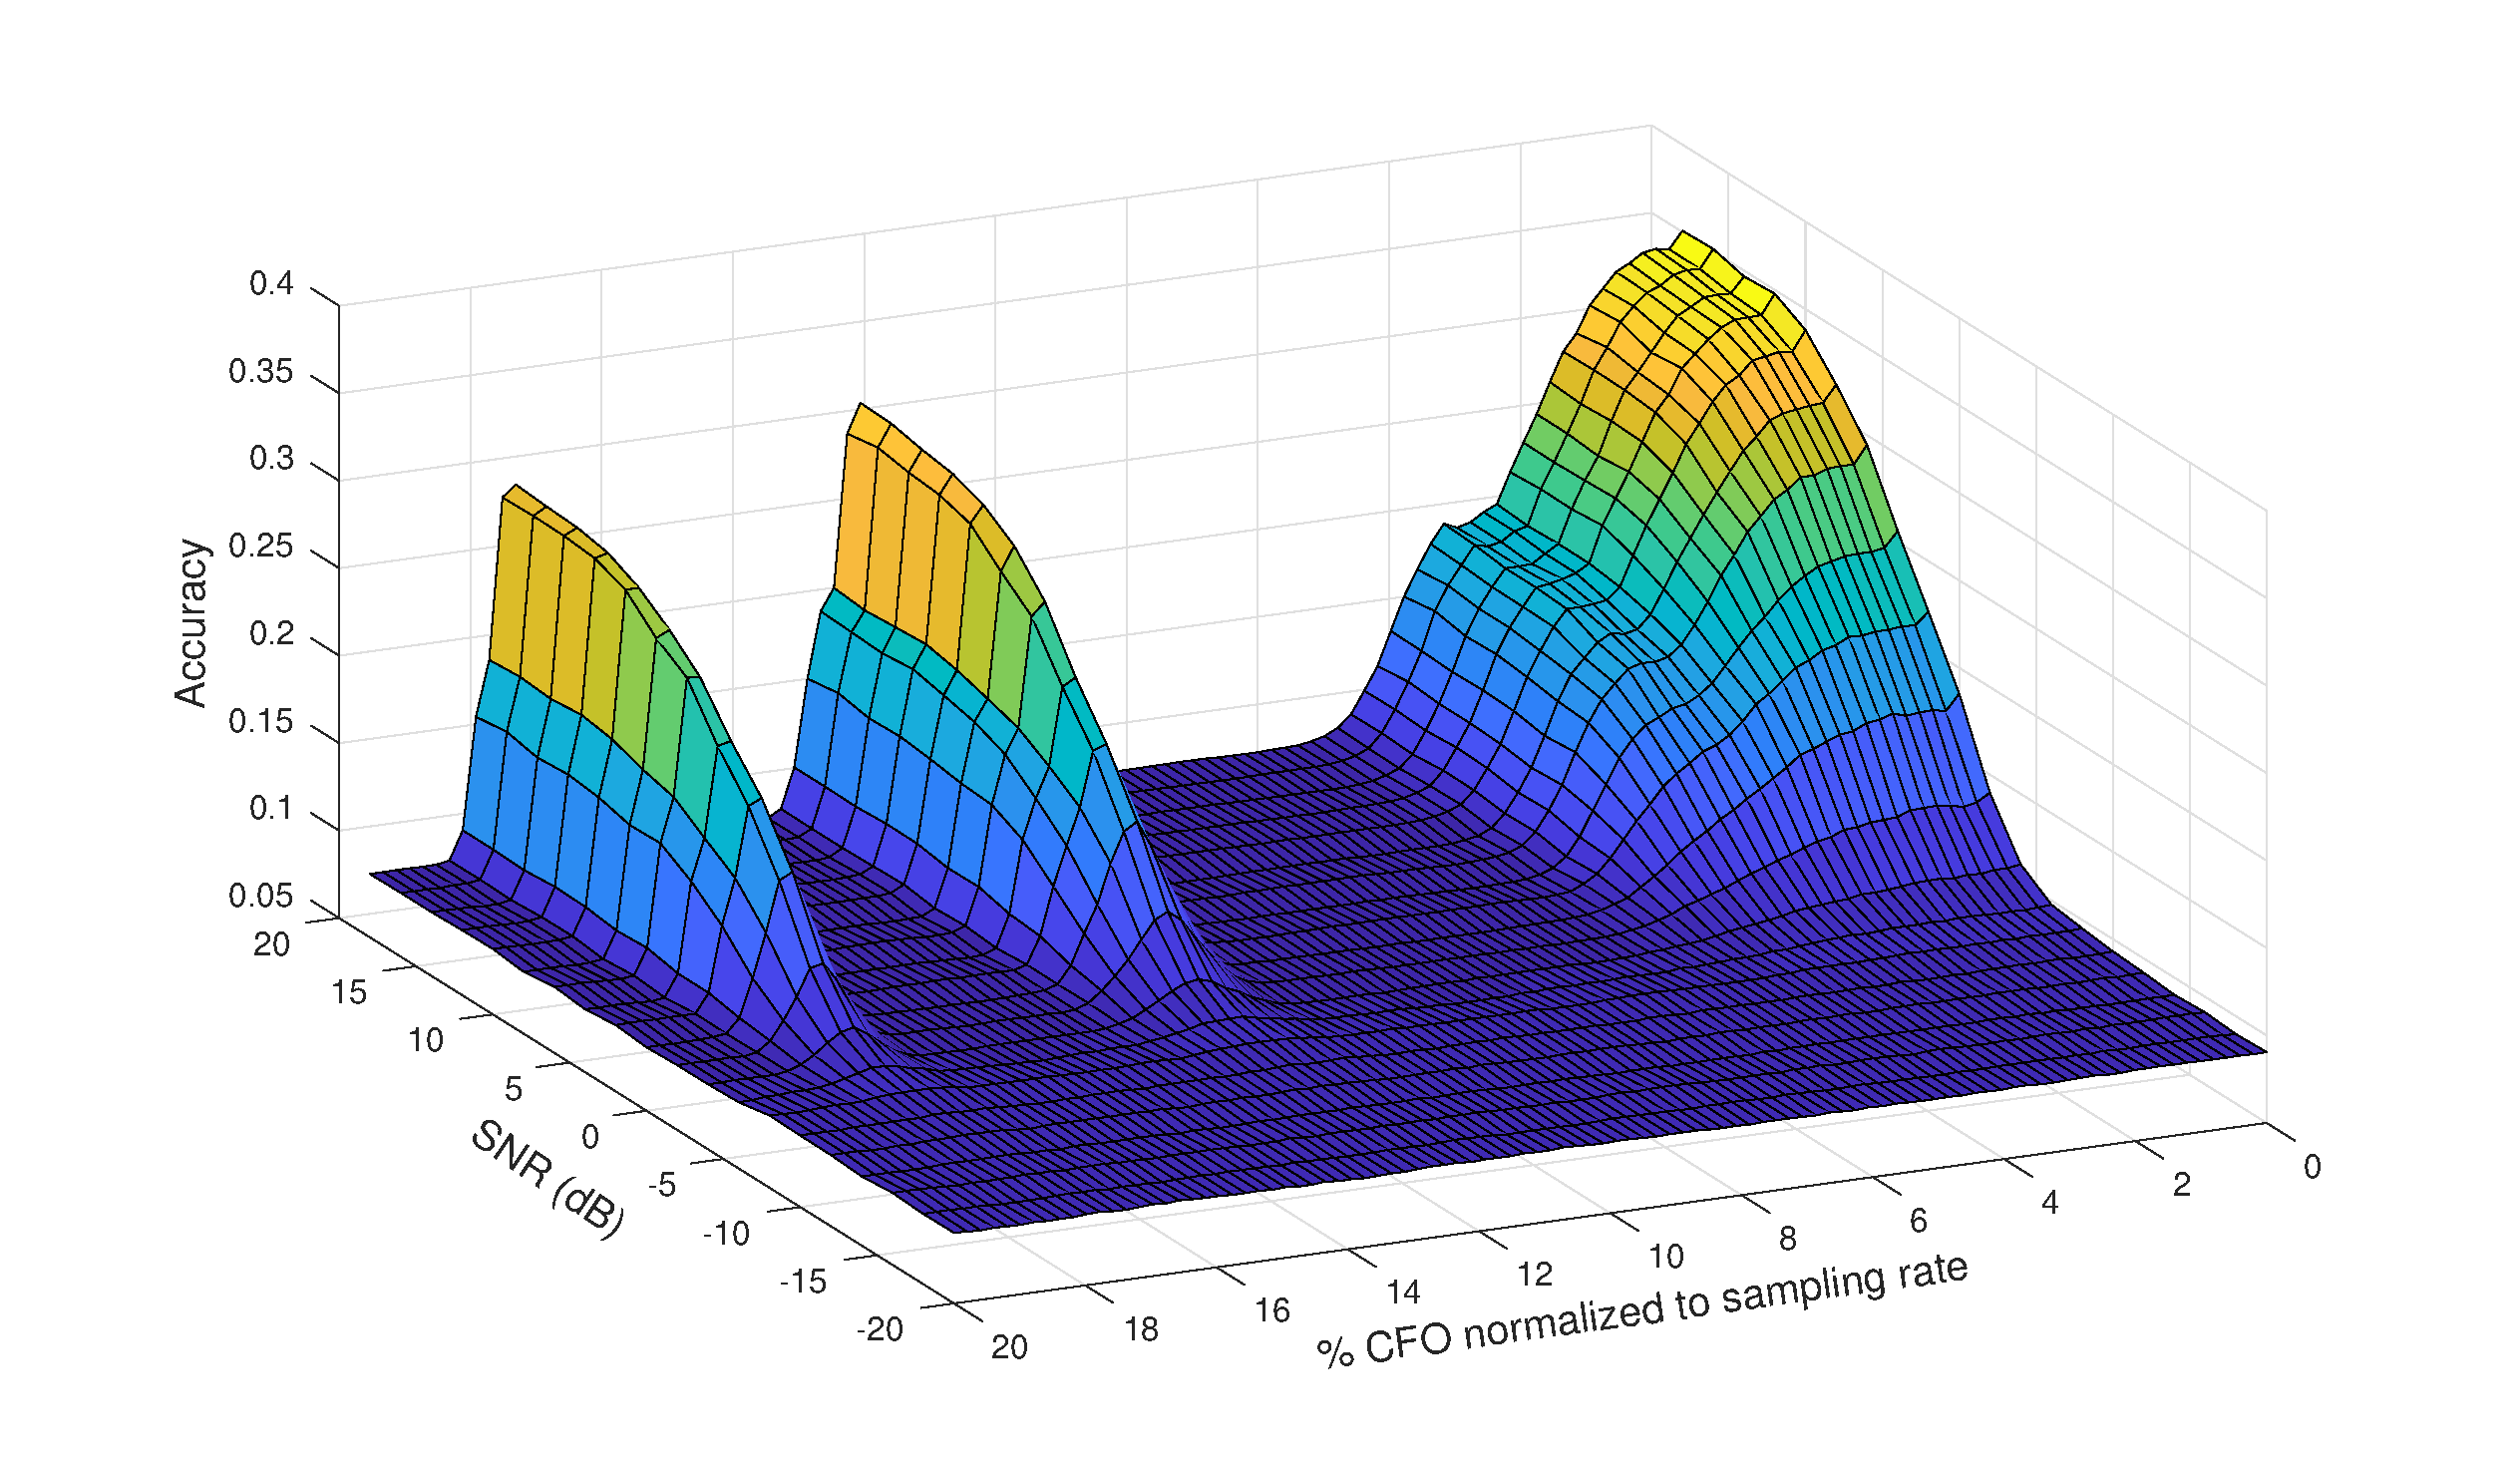
\includegraphics[width=0.45\textwidth,keepaspectratio]{figs/rml2016_tencfo.eps}
    \caption{CFO\_super test results when trained with CFO\_grc, as in the original 2016 dataset. Accuracy is averaged over 11 modulation schemes, and significantly decreases when tested against CFO channels of more than $1\%$ normalized to sample rate. Accuracy peaks at $38\%$.} 
\label{fig:cfo}      
\end{figure}

\begin{figure}[ht!]
	\centering	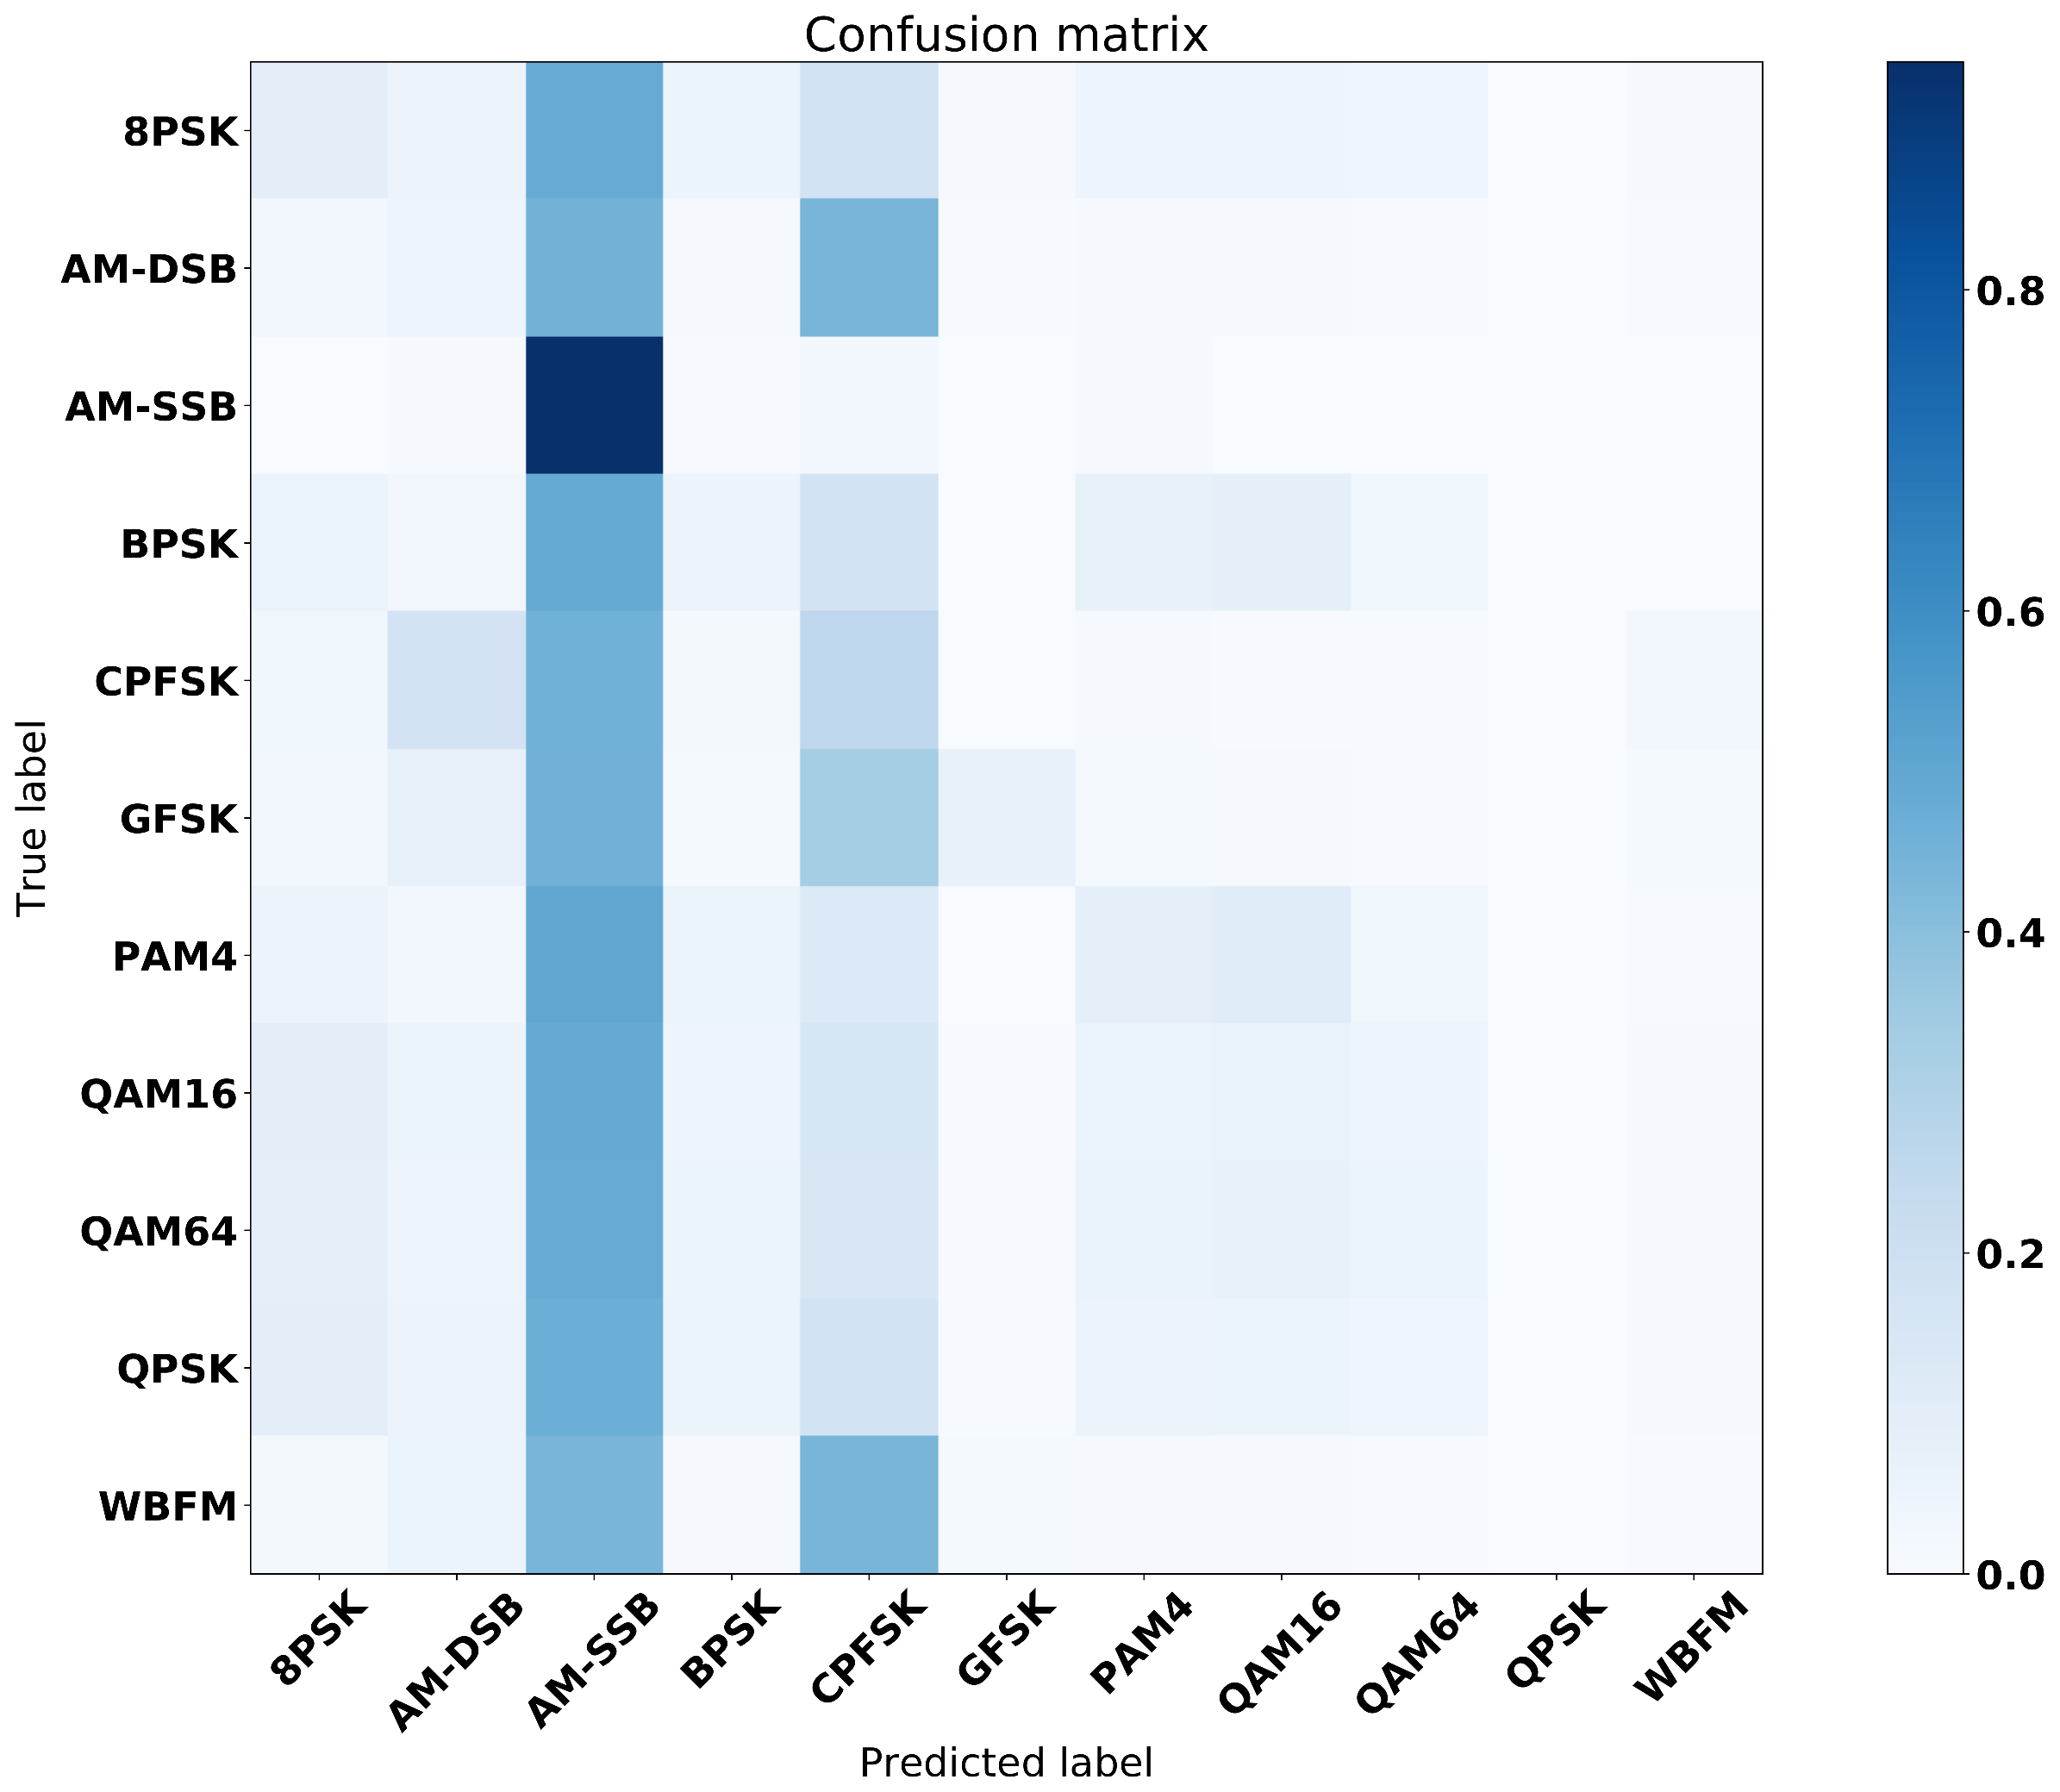
\includegraphics[width=0.45\textwidth,keepaspectratio]{figs/confusion.eps}
    \caption{CFO\_super confidence matrix for $12.53\%$ CFO averaged over SNR, see Figure~\ref{fig:cfo}. AM-SSB is the predicted label at low SNR values as when there is no CFO, and often correctly predicts CPFSK at higher SNR values. This seems to imply certain periodic CFO values do not affect the appearance of CPFSK constellation plots.} 
\label{fig:confusion}      
\end{figure}

Since the classifier is shown in confusion matrices to guess AM-SSB when SNR is low, resulting classifier accuracy nears $9.09\%$. The accuracy values peak when there is no CFO and sharply decreases as CFO grows in Figure~\ref{fig:nocfo}. The small improvement in accuracy at high SNR values and CFO values of $12.53\%$ and $17.78\%$ in Figure~\ref{fig:cfo} are due to the classifier correctly predicting the modulation scheme is Continuous Phase Frequency Shift Keying (CPFSK). Although accuracy improvement is small, if the classifier is only used to decide between CPFSK and a few other modulation schemes rather than 11, the accuracy increase would be much more significant, perhaps enough for the CFO correction to be relaxed or removed. Figure~\ref{fig:nocfo} reveals that the classifier does not perform with more than $0.2\%$ CFO when trained with RML\_4sps, which is problematic. Figure~\ref{fig:cfo} displays, as shown in~\cite{8170853}, the peak accuracy dropping due to the added complexity of the data from about $60\%$ to $40\%$, but that accuracy now stretches to $1\%$ CFO normalized to sample rate. A training decision here is to identify the CFO  (\ref{eq3}) of the system used in experimentation, and train the classifier for CFOs no greater than that to maintain peak accuracy.

Given the uniform distribution of initial phase offset in radio communications, Figure~\ref{fig:phase} reveals significant drops in accuracy at many phase offset values. Consequently, this classifier would likely require phase correction through either codewords, differential encoding, or equalization to see consistent near-peak performance.

\begin{figure}[ht!]
	\centering	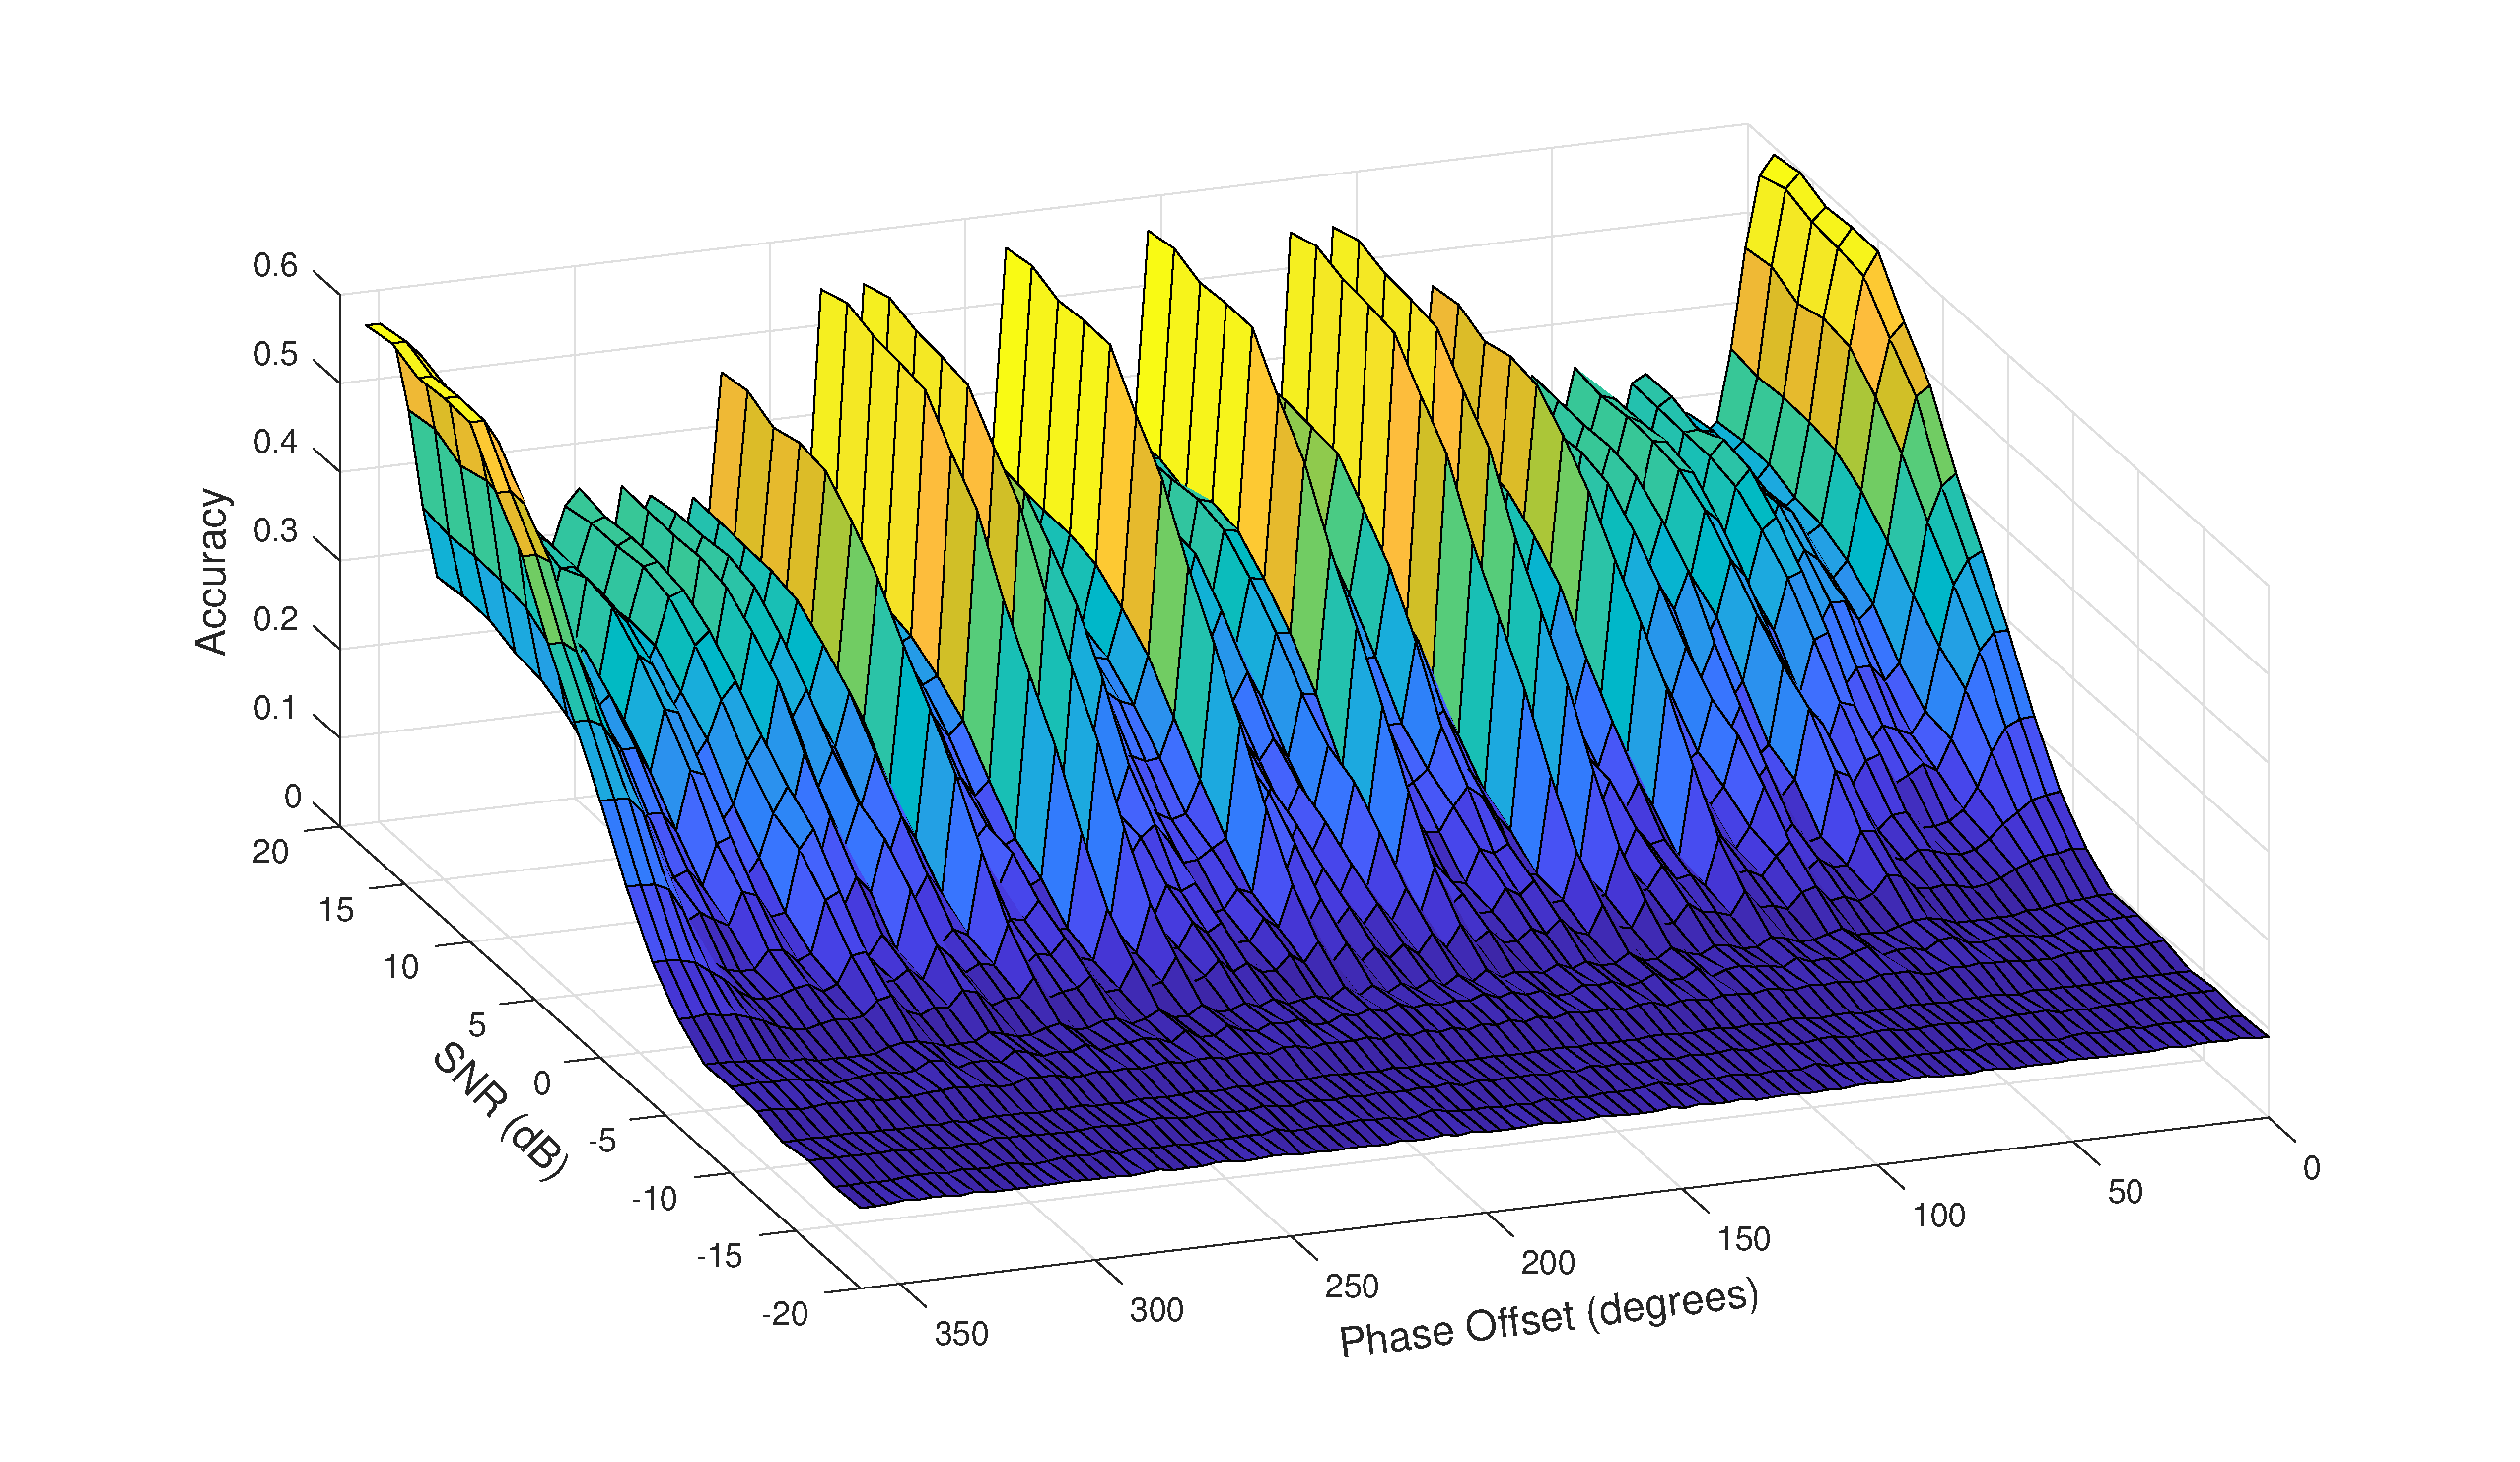
\includegraphics[width=0.45\textwidth,keepaspectratio]{figs/phase_sweep.eps}
    \caption{Phase\_super test results when trained with RML\_4sps. Accuracy is averaged over 11 modulation schemes, and remains close to peak performance for phase offsets of less than 4 degrees and certain discretized values. $60\%$ peak accuracy can drop by as much as half for many phase offset values.} 
\label{fig:phase}      
\end{figure}

\subsection{Summary}
\label{sec5}
In section~\ref{sec1}, we described the usefulness of NNs in the communications community, and referenced an overview of recent publications. In section~\ref{sec2} the frameworks's structure was discussed, and the implementation details of RadioML and our framework were visited in section~\ref{sec3}. Finally, section~\ref{sec4} displayed simulation results using NN datasets modified by our framework.

Our proposed framework showcases an ability to identify NN testing and training decisions, and hypothesize and test for answers to what extent training complexity should be taken for different wireless channel phenomenon. Future work aims to generate multi-user supersets from lists of DUTs, where channel blocks applied to different transmissions are related by correlation factors.


%% Heterogeneous CSS Implementation..
\chapter{Proposed LTE-R Channel Model and Framework}
\label{chapter4}

abstract

\section{test}
test

\section{Summary}
summary



%% Conclusion..
\chapter{Conclusion}
\label{conclusion}
test

\section{Research Outcomes}
test

\section{Future Work}
test


%%%%%%%%%%%%%%%%%%%%%%%%%%%%%%%% THE FINISH %%%%%%%%%%%%%%%%%%%%%%%%%%%%%%%
%SEE HERE for BIBTEX styles: http://www.cs.stir.ac.uk/~kjt/software/latex/showbst.html
\bibliographystyle{IEEEtran}
\bibliography{mybib}

\appendix
%\addtocontents{toc}{\protect\contentsline{chapter}{\protect\numberline{}Appendix:}{}{}}
\chapter{Data Synthesis Framework}
\section{Meta.py}
\begin{lstlisting}[breaklines]
#!/usr/bin/python3.5
"""
Created on Sep 22, 2017
@author: kwmcclintick

Meta class for testing ChannelPush.py, see respective classes for their documentation
"""

import warnings
import configparser
import ChannelTool
import sys
warnings.simplefilter(action='ignore', category=FutureWarning)
import h5py
warnings.resetwarnings()

if __name__ == '__main__':
    if len(sys.argv) < 4:
        print("Usage: ./program {HDF5 filename with data}")
        print("Exiting...")
        quit()
    else:
        filename = sys.argv[1]

    print('\n-------------------BOOTING META FILE-------------------')
    # data under test
    infile = h5py.File(filename, "r")
    print("DUT file information:")
    for item in infile.attrs.keys():
        print(item + ":", infile.attrs[item])

    datapath = infile.attrs['default']
    print("# of Symbols: " + str(int(len(infile[datapath]) / infile['source_data'].attrs['oversampling_factor'])))
    print("Samples Per Symbol: " + str(infile['source_data'].attrs['oversampling_factor']))
    print("# of Samples: " + str(len(infile[datapath])))

    # channelconfig gives instructions to the ChannelTool on what to test the data with
    # this is just printing out the contents of channelconfig
    channelconfig = configparser.ConfigParser()
    print("\n" + "Instructions File information:")
    print(str(channelconfig.read(str(sys.argv[2]))) + " Channels and Channel Characteristics have been loaded")
    for each_section in channelconfig.sections():
        print("[" + each_section + "]")
        for (each_key, each_val) in channelconfig.items(each_section):
            print(each_key + ":  " + each_val)

    output_tag = sys.argv[3]
    # ChannelTool multiplies input files by pushing them through different channels described by channelconfig
    ChannelTool = ChannelTool.ChannelTool(channelconfig, infile, output_tag)

    ChannelTool.run()

    # ChannelTool object created, file multiplication called
    print("\n" + "please wait, pushing samples through each channel series...")
    infile.close()

\end{lstlisting}

\section{ChannelPush.py}
\begin{lstlisting}[breaklines]
"""
Created on Oct, 10 2017
author: kwmcclintick
The ChannelTool class interacts with channel objects in mass, initializes information from ChannelConfig.ini,
and handles file multiplication by passing inputs through a variety of typical wireless channels with typical design
parameters
"""

import sys
import matplotlib.pyplot as plt
import os
from multiprocessing import Process, Pool
import numpy as np
import warnings
warnings.simplefilter(action='ignore', category=FutureWarning)
import h5py
warnings.resetwarnings()


class ChannelTool:
    def __init__(self, channelconfig, infile, output_tag):  # constructor
        print('\n-----------INITIALIZING DATASET SYNTHESIS FRAMEWORK----------')
        self.infile = infile
        self.output_tag = output_tag
        self.channelconfig = channelconfig

        # CREATING THE CHARACTERISTICS MATRIX FROM CHANNELCONFIG.INI
        print('////// CREATING 3D CHARACTERISTICS MATRIX //////')
        characteristics = self.charMatrix()

        # SEARCH CHANNELS FOLDER AND CREATE CHANNEL OBJECTS
        print('////// CREATING 2D MATRIX OF CHANNEL OBJECTS //////')
        self.channels = self.chanMatrix(characteristics)

    '''
    Running the ChannelTool picks one instance from each channel type and generates a data flow from those channels,
    modifying the input HDF5 file one channel at a time until saving the last channel's output as new HDF5 file with
    identifying attributes as to how the data was changed.
    '''
    def run(self):
        print('////// CREATING 1D CHANNEL SEQUENCES //////')
        channel_combos\
            = [list(x) for x in np.array(np.meshgrid(*self.channels)).T.reshape(-1, len(self.channels))]

        for k in range(len(channel_combos)):
            print("Starting channel data flow process " + str(k + 1) + " of " + str(len(channel_combos)))
            p = Process(target=self.dataFlow, args=(k, channel_combos[k],))
            p.start()

    '''
    Returns the first result in the directory path for the file of name name
    '''
    def find(self, name, path):
        for root, dirs, files in os.walk(path):
            if name in files:
                return os.path.join(root, name)

    '''
    attaches labels to the hdf5 outfile and writes it to the HDF5_files directory
    '''
    def dataFlow(self, k, channel_combos):
        # writing each hdf5 data set here
        outfile = h5py.File('./HDF5_files/noisyQPSK_' + str(k + 1) + self.output_tag + '.hdf5', "w")
        # point to the default data to be plotted
        outfile.attrs["default"] = "/out/bbIQ"  # group name/data set name
        # give the HDF5 root some more attributes, keeping group attributes same as input files (mod scheme, sps)
        outfile.attrs["Outfile_Name"] = 'noisyQPSK_' + str(k + 1) + self.output_tag
        outfile.attrs["creator"] = sys.argv[0]
        outfile.attrs["HDF5_Version"] = h5py.version.hdf5_version
        outfile.attrs["h5py_version"] = h5py.version.version
        outfile.attrs["modulation"] = self.infile['source_data'].attrs['modulation']
        outfile.attrs["oversampling_factor"] = self.infile['source_data'].attrs['oversampling_factor']

        # infile data is kept on hand for SER calculations and such
        source = outfile.create_group("source_data")
        source.create_dataset("bbIQ", data=self.infile[self.infile.attrs['default']])

        # each channels dash bigta flow computes here, attaching attributes to the hdf5 file as it goes
        outdata = self.labelPush(np.array(channel_combos, dtype=np.object), outfile)

        # initializing the hdf5 group that each data set will be written to
        grp = outfile.create_group("out")
        # file is actually written and closed
        grp.create_dataset("bbIQ", data=outdata)
        outfile.close()
        print('Closing hdf5 file: ' + str(k+1))

    '''
    Pushes data sample by sample through the kth sequence of channel_combos, attaching characteristic labels to hdf5
    outfile using attrs
    '''
    def labelPush(self, channel_combos, outfile):
        # single channel sequences
        if len(channel_combos) == 1:
            # attach labels
            for i in range(len(channel_combos[0].getCharacteristics())):
                outfile.attrs[str(channel_combos[0].characteristic_names[i])] \
                    = channel_combos[0].getCharacteristics()[i]
            channel_combos[0].compute()
            outdata = channel_combos[0].getOutput()

        # multiple channel sequences
        if len(channel_combos) > 1:
            for c in range(len(channel_combos) - 1):
                channel_combos[c].compute()
                channel_combos[c + 1].setInput(channel_combos[c].getOutput())
                # attach labels
                for i in range(len(channel_combos[c].getCharacteristics())):
                    outfile.attrs[str(channel_combos[c].characteristic_names[i])] \
                        = channel_combos[c].getCharacteristics()[i]
            # compute final channel output and attach final label
            channel_combos[len(channel_combos) - 1].compute()
            for i in range(len(channel_combos[c + 1].getCharacteristics())):
                outfile.attrs[str(channel_combos[c + 1].characteristic_names[i])] \
                    = channel_combos[c + 1].getCharacteristics()[i]
            outdata = channel_combos[len(channel_combos) - 1].getOutput()
        return outdata

    '''
    Creates a 3D characteristics matrix. Each channel has a list of characteristics, and each characteristic
    has a list of values it iterates through
    '''
    def charMatrix(self):
        num_channels = len(self.channelconfig.items(self.channelconfig.sections()[0]))
        characteristics = [[0 for x in range(1)] for y in range(num_channels)]
        for i in range(num_channels):
            # .ini files store values as strings, so I use a delimiter to separate the string into characteristics
            cur_chars = self.channelconfig['CHARACTERISTICS']['characteristics' + str(i + 1)].split('|')
            for k in range(len(cur_chars)):
                # and here again into separate values
                cur_chars[k] = cur_chars[k].split(',')
                # now everything is organized by characteristic and value, but are still strings. Here I parse as floats
                for b in range(len(cur_chars[k])):
                    cur_chars[k][b] = float(cur_chars[k][b])
            # finally we have our characteristics matrix for the i-th channel. We repeat again for each testing channel
            characteristics[i] = cur_chars
        return np.array(characteristics, dtype=np.object)

    '''
    Creates a 2D matrix of every possible combination of unique series of channel realizations from the
    characteristics 3D matrix and config file instructions
    '''
    def chanMatrix(self, characteristics):
        path = './Channels'
        # to initialize the channels, first I create a list of the names of testing channels
        channelsNames = self.channelconfig.items(self.channelconfig.sections()[0])
        channelsPaths = [None] * len(channelsNames)
        channels = [[0 for x in range(0)] for y in range(len(channelsNames))]
        # the list of channel names is iterated through and a list of channel objects is initialized according to
        # the list of channel names and the list of characteristics

        for i in range(len(channelsNames)):
            channelsNames[i] = channelsNames[i][1]
            channelsPaths[i] = self.find(channelsNames[i] + '.py', path)
            if channelsPaths[i] is None:
                sys.exit('Error: channel ' + channelsNames[i] + ' not found or not Python file')

        for i in range(len(channels)):
            # these channels have non-zero characteristics so a channel object is created for each combo of character
            self.combos = \
                [list(x) for x in
                 np.array(np.meshgrid(*characteristics[i])).T.reshape(-1, len(characteristics[i]))]
            for d in range(len(self.combos)):
                mod = __import__('Channels.' + channelsNames[i], globals(), locals(), channelsNames[i])
                class_ = getattr(mod, channelsNames[i])
                cur_channel = class_(self.combos[d], self.infile)
                if len(self.combos[d]) != len(cur_channel.getCharacteristic_names()):
                    print(len(self.combos[d]))
                    print(len(cur_channel.getCharacteristic_names()))
                    sys.exit('Error: channel ' + channelsNames[i] + ' has wrong number of characteristics')
                channels[i].insert(d, cur_channel)
        return channels

\end{lstlisting}

\section{merge\_datasets.py}
\begin{lstlisting}[breaklines]
#!/usr/bin/python3.5
"""
Created on Sep 22, 2017
@author: kwmcclintick

Meta class for testing ChannelTool.py, see respective classes for their documentation
"""

from pylab import *
import warnings
import math
import os
import configparser
from os import listdir
from os.path import isfile, join
import sys
warnings.simplefilter(action='ignore', category=FutureWarning)
import h5py
warnings.resetwarnings()


'''
modulate frequency shifts data to a specified Intermediate Frequency (IF)
modulated data = I*cos(2pi * fc * t) + Q*sin(2pi * fc * t)
where t = n*Ts where Ts = 1/Fs, sampling frequency, n is the nth sample
'''


def modulate(file, Fs, IF):
    print('\nModulating files...')
    data = file[file.attrs['default']]
    mod_data = [None] * len(data)

    # plt.magnitude_spectrum(data, Fs=50000000)
    # plt.title("Pulse Shaped AWGN Data-Set, IF = " + IF)
    # plt.show()

    phase_per_sample = 2*math.pi * float(IF) * 1/float(Fs)
    for i in range(len(data)):  # phase grows with each symbol, spinning the constellation with time
        curr_phase = phase_per_sample * (i + 1)
        new_real = data[i].real*math.cos(curr_phase)
        new_imag = data[i].imag*math.sin(curr_phase)
        new_imag = 0  # sampling must be real, not complex
        mod_data[i] = complex(new_real, new_imag)
    return mod_data


'''
sums the complex values of all files_to_sum
'''


def sum_files(data_to_sum):
    print("Summing files...")
    merged_data = [complex(0,0)] * len(data_to_sum[0][0])

    for each_dir in data_to_sum:
        for each_list in each_dir:
            for i in range(len(each_list)):
                merged_data[i] = merged_data[i] + each_list[i]
    return merged_data


if __name__ == '__main__':
    if len(sys.argv) < 5:
        print("Usage: ./program {HDF5 filename with data}")
        print("Exiting...")
        quit()
    else:
        # directory containing each IF sub directory
        dir = sys.argv[1]

    print('\n--------------MODULATING AND SUMMING DATASETS--------------')
    # list of IF sub directories IF1, IF2, etc.
    sub_dirs = [x[0] for x in os.walk(dir)]
    sub_dirs.pop(0)

    # mergeconfig gives instructions on what frequency to modulate which datasets up to
    mergeconfig = configparser.ConfigParser()
    print(str(mergeconfig.read(str(sys.argv[2]))) + " Intermediate Frequency mappings have been loaded")
    for each_section in mergeconfig.sections():
        print("[" + each_section + "]")
        for (each_key, each_val) in mergeconfig.items(each_section):
            print(each_key + ":  " + each_val)

    # save list of IFs, Fs's
    IF = [i[1] for i in mergeconfig.items(mergeconfig.sections()[0])]
    IFnames = [i[0] for i in mergeconfig.items(mergeconfig.sections()[0])]
    Fs = [i[1] for i in mergeconfig.items(mergeconfig.sections()[1])]

    # throw error if number of IF in config file != number of IF sub directories in argv[1]
    if len(sub_dirs) != len(mergeconfig.items(mergeconfig.sections()[0])):
        sys.exit('Error: number of IF in config file: ' + str(len(mergeconfig.items(mergeconfig.sections()[0]))) +
                 ' != number of IF sub directories in argv[1]: ' + str(len(sub_dirs)))

    # import all hdf5 files from the subdirectories
    merge_files = [None] * len(sub_dirs)
    i = 0
    for each_dir in sub_dirs:
        merged_file = None
        merge_files[i] = [f for f in listdir(each_dir) if isfile(join(each_dir, f))]
        for each_file in merge_files[i]:
            if not each_file.endswith('.hdf5'):
                merge_files[i].remove(each_file)
        # modulate each file to be merged
        print('\n///////// Directory: ' + str(each_dir) + ' /////////')
        j = 0
        for each_file in merge_files[i]:
            print('\n##### Target file: ' + str(each_file) + ' #####')
            print('HDF5 labels:')
            each_file = h5py.File(str(each_dir) + '/' + str(each_file), "r")

            # the order of directories isn't always the order of config values. Searches for subdirectory matching
            # the name of the key string in the config file
            freq_idx = IFnames.index(each_dir.split('/')[len(each_dir.split('/'))-1])

            for item in each_file.attrs.keys():
                print(item + ":", each_file.attrs[item])
            sps = each_file.attrs['oversampling_factor']
            each_file = modulate(each_file, Fs[freq_idx], IF[freq_idx])
            merge_files[i][j] = each_file
            j = j + 1
        i = i + 1

    # Sum all datasets from each directory after modulation
    merged_data = sum_files(merge_files)

    Fs = int(sys.argv[4])  # sampling frequency of receiving radio

    plt.magnitude_spectrum(merged_data, Fs=Fs)
    plt.title("Multi-transmission Data-Set Magnitude Response")
    plt.show()

    # writing each hdf5 data set here
    outfile = h5py.File('./merged_datasets/merged_set' + sys.argv[3] + '.hdf5', "w")
    # point to the default data to be plotted
    outfile.attrs["default"] = "/out/bbIQ"  # group name/data set name
    # give the HDF5 root some more attributes, keeping group attributes same as input files (mod scheme, sps)
    outfile.attrs["creator"] = sys.argv[0]
    outfile.attrs["HDF5_Version"] = h5py.version.hdf5_version
    outfile.attrs["h5py_version"] = h5py.version.version

    # initializing the hdf5 group that each data set will be written to
    grp = outfile.create_group("out")
    # file is actually written and closed
    grp.create_dataset("bbIQ", data=merged_data)
    outfile.close()
\end{lstlisting}

\section{upsampFilt.py}
\begin{lstlisting}[breaklines]
#!/usr/bin/python3

# kwmcclintick
# wilab

from pylab import *
import sys
import filters
import matplotlib.pyplot as plt
import numpy as np
import warnings
warnings.simplefilter(action='ignore', category=FutureWarning)
import h5py
warnings.resetwarnings()

if len(sys.argv) < 5:
	print("Usage: ./program {# of Symbols to make, SPS}")
	print("Exiting...")
	quit()
else:
	filename = sys.argv[1]
	infile = h5py.File(filename, "r")
	inputData = infile[infile.attrs['default']]
	rolloff_factor = float(sys.argv[2])
	span = int(sys.argv[3])
	sps = int(sys.argv[4])

print('\n----------------------UPSAMPFILT----------------------')
# separate inputData into real and imaginary parts
I = [None] * len(inputData)
Q = [None] * len(inputData)
for i in range(len(inputData)):
	I[i] = inputData[i].real
	Q[i] = inputData[i].imag

# interpolate
print("INTERPOLATING FILE BY: X" + str(sps))
N = sps  # up sampling factor, typed from float to int
interpolated_inputData_I = [0] * (len(I) * N)
interpolated_inputData_Q = [0] * (len(Q) * N)
for i in range(len(interpolated_inputData_I)):
	if i % N == 0:
		interpolated_inputData_I[i] = I[int(i / N)]
		interpolated_inputData_Q[i] = Q[int(i / N)]

# don't even ask, had to do some weird stuff to equate this filter class's rrcosfilter() function to MATLAB's
# wonderful rcosdesign() function
Ts = 10
Fs = N / 10
rrc_length = int(span * N + 2)  # filter length in samples, typed from float to int
# root raised cosine filter, h_rrc is the impulse response of the filter, time_idx the time values of h_rrc
time_idx, h_rrc = filters.rrcosfilter(rrc_length, rolloff_factor, Ts, Fs)
h_rrc = np.delete(h_rrc, 0)

# envelope is achieved by convolving the filters impulse response with our interpolated data
print("PULSE SHAPING FILE: rolloff: " + str(rolloff_factor) + ", sps: " + str(sps) + ", span: " + str(span))
filtered_inputData_I = np.convolve(interpolated_inputData_I, h_rrc, mode='full')
filtered_inputData_Q = np.convolve(interpolated_inputData_Q, h_rrc, mode='full')

#grpDelay = math.floor(len(h_rrc)/2)
outdata = [None] * int(len(filtered_inputData_I))  #- 2*grpDelay))
for i in range(len(outdata)):
	outdata[i] = complex(filtered_inputData_I[i], filtered_inputData_Q[i])

print(sys.argv[0][:2])
if sys.argv[0][:2] == "./":
	filestem = sys.argv[0][2:]
else:
	filestem = sys.argv[0]

filename = filestem[:-2] + "hdf5"
print(filename)

outfile = h5py.File(filename, "w")

I = [None] * len(outdata)
Q = [None] * len(outdata)
for i in range(len(outdata)):
	I[i] = outdata[i].real
	Q[i] = outdata[i].imag

plt.plot(I, Q, linewidth=0.1)
plt.title("8SPS Pulse Shaped Input I/Q")
plt.xlabel("Real")
plt.ylabel("Imaginary")
# plt.show()

# point to the default data to be plotted
outfile.attrs["default"]          = "/source_data/bbIQ"
# give the HDF5 root some more attributes
outfile.attrs["file_name"]        = filename
outfile.attrs["creator"]          = filestem
outfile.attrs["HDF5_Version"]     = h5py.version.hdf5_version
outfile.attrs["h5py_version"]     = h5py.version.version

dgroup = outfile.create_group("source_data")
dgroup.attrs["modulation"] = "QPSK"
dgroup.attrs["oversampling_factor"] = sps
dgroup.attrs["Beta"] = rolloff_factor
dgroup.create_dataset("bbIQ", data=outdata)

outfile.close()
\end{lstlisting}

\section{Filtdownsamp.py}
\begin{lstlisting}[breaklines]
#!/usr/bin/python3

# kwmcclintick
# wilab

import sys
import filters
import math
import matplotlib.pyplot as plt
import numpy as np
import warnings
warnings.simplefilter(action='ignore', category=FutureWarning)
import h5py
warnings.resetwarnings()

if len(sys.argv) < 5:
	print("Usage: ./program {# of Symbols to make, SPS}")
	print("Exiting...")
	quit()
else:
	filename = sys.argv[1]
	infile = h5py.File(filename, "r")
	inputData = infile[infile.attrs['default']]
	rolloff_factor = float(sys.argv[2])
	span = int(sys.argv[3])
	sps = int(sys.argv[4])

print('-------------------FILTDOWNSAMP-------------------')

# separate inputData into real and imaginary parts
I = [None] * len(inputData)
Q = [None] * len(inputData)
for i in range(len(inputData)):
	I[i] = inputData[i].real
	Q[i] = inputData[i].imag

# don't even ask, had to do some weird stuff to equate this filter class's rrcosfilter() function to MATLAB's
# wonderful rcosdesign() function
N = sps  # up sampling factor, typed from float to int
Ts = 10
Fs = N / 10
rrc_length = int(span * N + 2)  # filter length in samples, typed from float to int
# root raised cosine filter, h_rrc is the impulse response of the filter, time_idx the time values of h_rrc
time_idx, h_rrc = filters.rrcosfilter(rrc_length, rolloff_factor, Ts, Fs)
h_rrc = np.delete(h_rrc, 0)

print("MATCHED FILTERING FILE: rolloff: " + str(rolloff_factor) + ", sps: " + str(sps) + ", span: " + str(span))

# envelope is achieved by convolving the filters impulse response with our interpolated data
filtered_inputData_I = np.convolve(I, h_rrc, mode='full')
filtered_inputData_Q = np.convolve(Q, h_rrc, mode='full')

print("DECIMATING FILE BY: X" + str(sps))
# decimate
decimated_I = [0] * int((len(filtered_inputData_I) / N) - len(h_rrc))
decimated_Q = [0] * int((len(filtered_inputData_I) / N) - len(h_rrc))
for i in range(len(decimated_I)):
	decimation_index = int(math.floor(len(h_rrc) / 2) + (i * N))
	decimated_I[i] = filtered_inputData_I[decimation_index]
	decimated_Q[i] = filtered_inputData_Q[decimation_index]

outdata = [None] * len(decimated_Q)
for i in range(len(decimated_Q)):
	outdata[i] = complex(decimated_I[i], decimated_Q[i])

print(sys.argv[0][:2])
if sys.argv[0][:2] == "./":
	filestem = sys.argv[0][2:]
else:
	filestem = sys.argv[0]

filename = filestem[:-2] + "hdf5"
print(filename)

outfile = h5py.File(filename, "w")

I = [None] * len(outdata)
Q = [None] * len(outdata)
for i in range(len(outdata)):
	I[i] = outdata[i].real
	Q[i] = outdata[i].imag

plt.scatter(I,Q)
plt.title("Match Filtered, Downsampled I/Q")
plt.xlabel("Real")
plt.ylabel("Imaginary")
plt.show()

# point to the default data to be plotted
outfile.attrs["default"]          = "/source_data/bbIQ"
# give the HDF5 root some more attributes
outfile.attrs["file_name"]        = filename
outfile.attrs["creator"]          = filestem
outfile.attrs["HDF5_Version"]     = h5py.version.hdf5_version
outfile.attrs["h5py_version"]     = h5py.version.version

dgroup = outfile.create_group("source_data")
dgroup.attrs["modulation"] = "QPSK"
dgroup.attrs["oversampling_factor"] = sps
dgroup.attrs["Beta"] = rolloff_factor
dgroup.create_dataset("bbIQ", data=outdata)

outfile.close()
\end{lstlisting}

\section{Channel.py}
\begin{lstlisting}[breaklines]
"""
Created on Sep 22, 2017
@author: kwmcclintick

The Channel parent class contains methods and instance variables that all wireless channel
blocks should share. Any wireless channel should of course have a name so it can be identified,
inputs and outputs (as any system has), a README so insight can be gained about the class without
diving into it's .py file, and characteristics with which the channel can apply to the input in
its computeOutput method.
"""

import numpy as np


class Channel:

    def __init__(self, name, characteristics, infile):  # constructor
        self.characteristic_names = [None]
        self.name = name
        self.characteristics = characteristics
        self.infile = infile
        self.inputData = np.array(list(self.infile[self.infile.attrs['default']]), dtype=np.complex)
        self.outputData = [0] * len(self.inputData)
        
    def getName(self):  # get method to return instance variable
        return self.name
    
    def getInput(self):  # get method to return instance variable
        return self.inputData
    
    def getOutput(self):  # get method to return instance variable
        return self.outputData

    def getCharacteristics(self):  # get method to return instance variable
        return self.characteristics

    def getCharacteristic_names(self):
        return self.characteristic_names
    
    def README(self):  # get method to return instance variable
        return self.readme

    def setInput(self, newInput):  # set method used in ChannelTool.py
        self.inputData = newInput

    def setCharacteristics(self, characteristics):
        self.characteristics = characteristics

    def setInfile(self, infile):
        self.infile = infile
\end{lstlisting}

\section{AWGNFriis.py}
\begin{lstlisting}[breaklines]
"""
Created on Sep 22, 2017
@author: kwmcclintick

AWGNFriis is a channel child class that represents how an Additive White Gaussian Noise wireless
channel modifies information passed through it using the Friis formula and Boltzmann
"""

import warnings
warnings.filterwarnings("ignore", message="numpy.dtype size changed")
warnings.filterwarnings("ignore", message="numpy.ufunc size changed")
from random import gauss
from pylab import *
from Channels.Channel import Channel
import matplotlib.pyplot as plt
from scipy import signal
from pylab import plot, xlabel, ylabel, ylim, title, show


class AWGNFriis(Channel):
    
    def __init__(self, characteristics, infile):  # constructor
        # parent's constructor is called. Everything else in here should be specific to the AWGN child class
        Channel.__init__(self, type(self).__name__, characteristics, infile)

        # this is used in write_to_hdf5 to create attributes for the output data set
        self.characteristic_names = ["bandwidth", "temp", "Ptx", "Gtx", "Grx", "d", "lambda", "Lsys", "Fs"]

    '''
    compute_write is the function called when a new process is created. Everything in this function is done in parallel
    with other combinations of channel characteristics

    AWGN's compute output adds zero mean Gaussian distributed real and imaginary numbers to
    the input QI data. The real and imaginary parts of the noise are statistically independent.
    The variance and amplitude of the noise is user specified with variables var and SNR.

    The more oversampling there is, the more the AWGN noise is reduced for each sample
    '''
    def compute(self):
        bandwidth = self.characteristics[0]
        temp = self.characteristics[1]
        Ptx = self.characteristics[2]
        Gtx = self.characteristics[3]
        Grx = self.characteristics[4]
        d = self.characteristics[5]
        lamb = self.characteristics[6]
        Lsys = self.characteristics[7]
        Fs = self.characteristics[8]
        # Friis eq, Power received in dB
        Lpath = 10*math.log10((4 * math.pi * d / lamb)**2)
        PrxdB = 10*math.log10(Ptx/0.001) + Gtx + Grx - Lpath - Lsys
        Prx = 10**(PrxdB / 10)

        Pnoise = 0.00000000245  # noise power in watts, measured by K. Gill with an N210 in our lab AK318
        # 450 MHz 7.5 kHz bin size
        #Pnoise = 10*math.log10(Pnoise)
        snr = Prx / Pnoise
        snrdB = 10*math.log10(snr)

        k = 1.38 * 10**-23  # Boltzmann constant
        h = 6.62 * 10**-34  # Planck constant
        R = 50  # resistance of SMA port, ohms
        variance = 2*(math.pi*k*temp)**2 / (3 * h) * R * bandwidth**0.5

        Asig_rms = 0
        sps = self.infile['source_data'].attrs['oversampling_factor']

        # here, input data is looped through to find the rms amplitude so that the noise amplitude can
        # appropriately be determined
        for b in range(len(self.inputData)):
            Asigcurrent = math.sqrt(pow(self.inputData[b].real, 2) + pow(self.inputData[b].imag, 2))
            Asig_rms += math.pow(Asigcurrent, 2)
        Asig_rms = math.sqrt((1 / (b + 1)) * Asig_rms)

        awgnNoise = [0] * len(self.inputData)
        for i in range(len(self.inputData)):
            # noise amplitude of each symbol in log scale
            awgnNoise[i] = Asig_rms * 10 ** (-snrdB / 20.0) * complex(gauss(0, math.sqrt(variance)),
                                                                   gauss(0, math.sqrt(variance)))
            # limit noise amplitude by SPS
            awgnNoise[i] = awgnNoise[i] / sps
        # band-limit the AWGN noise
        band_limited_noise = self.bandLimit(bandwidth, Fs, awgnNoise)
        # apply band-limited noise to input data
        for i in range(len(self.outputData)):
            self.outputData[i] = self.inputData[i] + band_limited_noise[i]

    '''
    Applies a 1001-order Blackman Harris Low Pass Filter to the AWGN list of values to keep all spectral noise in-band
    with the signal to prevent machine learning tricks
    '''
    def bandLimit(self, bandwidth, Fs, noise):
        # plot incoming noise magnitude response
        # plt.magnitude_spectrum(noise, Fs=Fs)
        # plt.title("Noise Magnitude Response")
        # plt.show()

        n = 1001  # filter order
        half_n = int(math.floor(n/2))
        cutoff = bandwidth / Fs

        # Lowpass filter defined
        a = signal.firwin(n, cutoff, window='blackmanharris')
        band_limtited_AWGN = np.convolve(noise, a, mode='full')
        for i in range(half_n, len(noise) + half_n):
            band_limtited_AWGN[i - half_n] = band_limtited_AWGN[i]
        '''
        plot filter impulse response
        stem(a)
        title("Blackman Harris LPF Impulse Response")
        show()

        plot filter frequency response
        plt.magnitude_spectrum(band_limtited_AWGN, Fs=Fs)
        plt.title("band_limtited_AWGN Magnitude Response")
        plt.show()
        
        b = a  # coeffecients, numerator
        a = 1  # coeffecients, denominator
        w, h = signal.freqz(b, a)
        h_dB = 20 * log10(abs(h))
        subplot(211)
        plot(w / max(w), h_dB)
        ylim(-150, 5)
        ylabel('Magnitude (db)')
        xlabel(r'Normalized Frequency (x$\pi$rad/sample)')
        title(r'Frequency response')
        subplot(212)
        h_Phase = unwrap(arctan2(imag(h), real(h)))
        plot(w / max(w), h_Phase)
        ylabel('Phase (radians)')
        xlabel(r'Normalized Frequency (x$\pi$rad/sample)')
        title(r'Phase response')
        subplots_adjust(hspace=0.5)
        show()
        '''

        return band_limtited_AWGN
\end{lstlisting}

\section{STOresolution.py}
\begin{lstlisting}[breaklines]
"""
Created on Nov 17, 2017
@author: kwmcclintick

Symbol Timing Offset (STO) is a channel child class that simulates timing error by interpolating data up the smallest
intermediate SPS needed to achieve a certain % of a symbol offset. A 4 sps signal, could, for instance, have an
offset of 0 (0% offset), 1 (25% offset), 2 (50% offset), or 3 (75% offset). If the resolution desired is 0.125,
the intermediate SPS would be 2, and 4 if the resolution desired was 0.0625, and so on.

the timing offset is random but constant for each transmission.
"""

import warnings
warnings.filterwarnings("ignore", message="numpy.dtype size changed")
warnings.filterwarnings("ignore", message="numpy.ufunc size changed")
from Channels.Channel import Channel
import matplotlib.pyplot as plt
import numpy as np
import math
import numpy
from numpy import abs
from scipy import signal


class STOresolution(Channel):
    def __init__(self, characteristics, infile):  # constructor
        # parent's constructor is called. Everything else in here should be specific to the AWGN child class
        Channel.__init__(self, type(self).__name__, characteristics, infile)

        # this is used in write_to_hdf5 to create attributes for the output data set
        self.characteristic_names = ["resolution"]

    '''
    compute_write is the function called when a new process is created. Everything in this function is done in parallel
    with other combinations of channel characteristics
    '''
    def compute(self):
        sps = self.infile['source_data'].attrs['oversampling_factor']
        resolution = float(self.characteristics[0])

        # interpolation filter defined
        # ~~[Filter Design with Parks-McClellan Remez]~~
        order = 32  # Filter order
        # Filter symetric around 0.25 (where .5 is pi or Fs/2)
        bands = numpy.array([0., .22, .28, .5])
        h = signal.remez(order + 1, bands, [1, 0], [1, 1])
        h[abs(h) <= 1e-4] = 0.
        # (w, H) = signal.freqz(h)  # quicker falloff, higher dB stop band

        # ~~[Filter Design with Windowed freq]~~
        # b = signal.firwin(order + 1, 0.5)
        # b[abs(h) <= 1e-4] = 0.
        # (wb, Hb) = signal.freqz(b)  # slower falloff, lower dB stop band

        if (1/sps) / resolution == 0:  # offset determined as in STOauto.py if sps is sufficient to achieve res
            offset = round(np.random.uniform(0, sps))
            for i in range(len(self.inputData) - offset):
                self.outputData[i] = self.inputData[i + offset]
        else:
            counter = sps
            # data is temp upsampled and filtered with an interpolation filter then downsampled such that the new
            # sps is a multiple of the original and the resolution achieved is less than or equal to the desired
            while (1/counter) > resolution or counter % sps != 0:
                counter += 1

            N = int(counter/sps)  # our temp interpolation decimation rate
            iteration = N  # if N = 8, this loop will interp by 2, filter 3 times, to get a total 2*2*2 = 8
            N = 2  # each iteration will interpolate by 2

            # separate inputData into real and imaginary parts
            I = [None] * len(self.inputData)
            Q = [None] * len(self.inputData)
            for i in range(len(self.inputData)):
                I[i] = self.inputData[i].real
                Q[i] = self.inputData[i].imag

            # plt.stem(I)
            # plt.title("input pulse shaped data")
            # plt.xlabel("sample #")
            # plt.ylabel("amplitdue")
            # plt.show()

            # interpolate
            interpolated_inputData_I = [0] * (len(I) * N)
            interpolated_inputData_Q = [0] * (len(Q) * N)
            for i in range(len(interpolated_inputData_I)):
                if i % N == 0:
                    interpolated_inputData_I[i] = I[int(i / N)]
                    interpolated_inputData_Q[i] = Q[int(i / N)]

            # plt.stem(interpolated_inputData_I)
            # plt.title("interpolated_inputData_I")
            # plt.xlabel("sample #")
            # plt.ylabel("amplitdue")
            # plt.show()

            # envelope is achieved by convolving the filters impulse response with our interpolated data
            filtered_inputData_I = np.convolve(interpolated_inputData_I, h, mode='full')
            filtered_inputData_Q = np.convolve(interpolated_inputData_Q, h, mode='full')

            # plt.stem(filtered_inputData_I)
            # plt.title("filtered_inputData_I")
            # plt.xlabel("sample #")
            # plt.ylabel("amplitdue")
            # plt.show()

            # interpolate and filter until the desired resolution is achieved
            iteration = iteration / 2
            while iteration != 1:
                # interpolate again
                interpolated_inputData_I = [0] * (len(filtered_inputData_I) * N)
                interpolated_inputData_Q = [0] * (len(filtered_inputData_Q) * N)
                for i in range(len(interpolated_inputData_I)):
                    if i % N == 0:
                        interpolated_inputData_I[i] = filtered_inputData_I[int(i / N)]
                        interpolated_inputData_Q[i] = filtered_inputData_Q[int(i / N)]

                # filter again
                filtered_inputData_I = np.convolve(interpolated_inputData_I, h, mode='full')
                filtered_inputData_Q = np.convolve(interpolated_inputData_Q, h, mode='full')

                iteration = iteration / 2  # iteration is changed to signal a 2x interp and filtering loop

            # apply symbol timing offset
            offset = np.random.randint(0, sps * int(counter/sps) - 1)
            for i in range(len(filtered_inputData_I) - offset):
                filtered_inputData_I[i] = filtered_inputData_I[i + offset]
                filtered_inputData_Q[i] = filtered_inputData_Q[i + offset]

            # plt.stem(filtered_inputData_I)
            # plt.title("offset filtered_inputData_I by: +" + str(offset) + " samp")
            # plt.xlabel("sample #")
            # plt.ylabel("amplitdue")
            # plt.show()

            N = int(counter / sps)  # our temp interpolation decimation rate
            for i in range(len(self.outputData)):
                decimation_index = int(math.log(N, 2)*math.floor(len(h) / 2) + (i * N))
                # decimated values are scaled according to the interpolation filter's max amplitude and the number
                # of times it was applied
                self.outputData[i] = complex((1/max(h))*math.log(N, 2)*filtered_inputData_I[decimation_index],
                                             (1 / max(h)) * math.log(N, 2)*filtered_inputData_Q[decimation_index])

            # plt.stem(decimatied_I, 'r-')
            # plt.stem(I)
            # plt.title("decimatied_I (red) vs. input I")
            # plt.xlabel("sample #")
            # plt.ylabel("amplitdue")
            # plt.show()
\end{lstlisting}

\section{RandomInitialPhase.py}
\begin{lstlisting}[breaklines]
"""
Created on Nov 14, 2017
@author: kwmcclintick

RandomInitialPhase is a channel child class that represents how a wireless transmitter can randomize the phase of
transmitted IQ data, since its exact distance as a multiple of carrier wavelength from the receiver is not
always considered.

The only difference between RandomInitialPhase and ClarkeScattering is that RandomInitialPhase applies the same
random phase to every symbol, while ClarkeScattering applies a different random phase to each symbol
"""

from Channels.Channel import Channel
import numpy as np
import math

class RandomInitialPhase(Channel):
    def __init__(self, characteristics, infile):  # constructor
        # parent's constructor is called. Everything else in here should be specific to the AWGN child class
        Channel.__init__(self, type(self).__name__, characteristics, infile)

    '''
    compute_write is the function called when a new process is created. Everything in this function is done in parallel
    with other combinations of channel characteristics
    '''
    def compute(self):
        theta = np.random.uniform(0, 2 * math.pi)
        phase = complex(math.cos(theta), math.sin(theta))
        for i in range(len(self.inputData)):
            self.outputData[i] = phase * self.inputData[i]
\end{lstlisting}

\section{IQimbalance.py}
\begin{lstlisting}[breaklines]
"""
Created on Nov 14, 2017
@author: kwmcclintick

IQimbalance is a channel child class that damages IQ symbols due to internal noise from an RF frontend. The idea
stems from the fact that the I and Q branches of an analog system will not have the same phase and magnitude as each
other.

This type of balance is assumed to be caused by a MIXER MISMATCH in a DIRECT UP transmit chain, and
is CONSTANT WITH RESPECT TO FREQUENCY

kI: in-phase magnitude, linear. ex: 0dB would give kI = 1
kQ: quadrature magnitude, linear.
phi_epsilon: phase difference, degrees

The channel is described by the matrix equation below

[sI] = [      kI               0      ] [sI']
[sQ]   [-kQsin(phi_ep)   kQcos(phi_ep)] [sQ']

where sI' and sQ' are the input IQ waveforms and sI and sQ are the output IQ waveforms after being damaged

this relationship should make it clear that a balanced system would have kI=kQ=1 and phi_epsilon=0, as sI=sI' and sQ=sQ'
"""

from Channels.Channel import Channel
import numpy


class IQimbalance(Channel):
    def __init__(self, characteristics, infile):  # constructor
        # parent's constructor is called. Everything else in here should be specific to the AWGN child class
        Channel.__init__(self, type(self).__name__, characteristics, infile)

        # this is used in write_to_hdf5 to create attributes for the output data set
        self.characteristic_names = ["k_I", "k_Q", "phi_epsilon"]

    '''
    compute_write is the function called when a new process is created. Everything in this function is done in parallel
    with other combinations of channel characteristics
    '''
    def compute(self):
        self.characteristics[2] = self.characteristics[2] * numpy.pi / 180.0  # converts phi_epsilon to radians

        for i in range(len(self.inputData)):
            self.outputData[i] = complex(self.characteristics[0]*self.inputData[i].real,
                                         self.inputData[i].imag*self.characteristics[1]*numpy.cos(self.characteristics[2])
                                         - self.inputData[i].real*self.characteristics[1]*numpy.sin(self.characteristics[2]))
\end{lstlisting}

\section{CFO.py}
\begin{lstlisting}[breaklines]
"""
Created on Nov 17, 2017
@author: kwmcclintick

Carrier Frequency Offset (CFO) is a channel child class that simulates small errors in the carrier frequency. The result
is each sample is rotated by a small phase value that builds with each sample, resulting in a spinning effect over
time of the IQ data based on the term fo/Fs

CFO.py is different than CFOSymRate.py in that CFO.py tries to model two independent Local Oscillators. A random
frequency offset is generated, and kept constant for each transmission.

A more accurate version of this model would include drift, varying the frequency offset even within each small
transmission
"""

from Channels.Channel import Channel
import math, random


class CFO(Channel):
    def __init__(self, characteristics, infile):  # constructor
        # parent's constructor is called. Everything else in here should be specific to the AWGN child class
        Channel.__init__(self, type(self).__name__, characteristics, infile)

        # this is used in write_to_hdf5 to create attributes for the output data set
        self.characteristic_names = ["Fc", "Fs", "PPM"]

    '''
    compute_write is the function called when a new process is created. Everything in this function is done in parallel
    with other combinations of channel characteristics
    '''
    def compute(self):
        Fc = self.characteristics[0]
        Fs = self.characteristics[1]
        PPM = self.characteristics[2]
        sps = self.infile['source_data'].attrs['oversampling_factor']

        # Tx and Rx both randomly choose an offset for each transmission of mean fc and std dev fo,max
        fo_max = PPM * Fc / 10**6
        std_dev = fo_max
        # bounded by fo,max, offset is re-picked if too large or too small
        fo_tx = random.gauss(0, std_dev)
        fo_rx = random.gauss(0, std_dev)
        while fo_rx < -fo_max or fo_rx > fo_max:
            fo_rx = random.gauss(0, std_dev)
        while fo_tx < -fo_max or fo_tx > fo_max:
            fo_tx = random.gauss(0, std_dev)

        # sum the offsets, worst case to_rx = to_tx = fo_max or -fo_max, best case both equal zero or opposite signs
        fo_total = fo_tx + fo_rx

        phase_per_sample = (2 * math.pi * fo_total / Fs) / sps

        for i in range(len(self.inputData)):  # phase grows with each symbol, spinning the constellation with time
            phase = phase_per_sample * (i + 1)
            rotation = complex(math.cos(phase), math.sin(phase))
            self.outputData[i] = rotation * self.inputData[i]
\end{lstlisting}

\section{filters.py}
\begin{lstlisting}[breaklines]

# Authors: Veeresh Taranalli <veeresht@gmail.com>
# License: BSD 3-Clause

"""
============================================
Pulse Shaping Filters (:mod:`commpy.filters`)
============================================

.. autosummary::
   :toctree: generated/

   rcosfilter          -- Raised Cosine (RC) Filter.
   rrcosfilter         -- Root Raised Cosine (RRC) Filter.
   gaussianfilter      -- Gaussian Filter.
   rectfilter          -- Rectangular Filter.

"""

import numpy as np

__all__=['rcosfilter', 'rrcosfilter', 'gaussianfilter', 'rectfilter']

def rcosfilter(N, alpha, Ts, Fs):
    """
    Generates a raised cosine (RC) filter (FIR) impulse response.

    Parameters
    ----------
    N : int
        Length of the filter in samples.

    alpha : float
        Roll off factor (Valid values are [0, 1]).

    Ts : float
        Symbol period in seconds.

    Fs : float
        Sampling Rate in Hz.

    Returns
    -------

    h_rc : 1-D ndarray (float)
        Impulse response of the raised cosine filter.

    time_idx : 1-D ndarray (float)
        Array containing the time indices, in seconds, for the impulse response.
    """

    T_delta = 1/float(Fs)
    time_idx = ((np.arange(N)-N/2))*T_delta
    sample_num = np.arange(N)
    h_rc = np.zeros(N, dtype=float)

    for x in sample_num:
        t = (x-N/2)*T_delta
        if t == 0.0:
            h_rc[x] = 1.0
        elif alpha != 0 and t == Ts/(2*alpha):
            h_rc[x] = (np.pi/4)*(np.sin(np.pi*t/Ts)/(np.pi*t/Ts))
        elif alpha != 0 and t == -Ts/(2*alpha):
            h_rc[x] = (np.pi/4)*(np.sin(np.pi*t/Ts)/(np.pi*t/Ts))
        else:
            h_rc[x] = (np.sin(np.pi*t/Ts)/(np.pi*t/Ts))* \
                    (np.cos(np.pi*alpha*t/Ts)/(1-(((2*alpha*t)/Ts)*((2*alpha*t)/Ts))))

    return time_idx, h_rc

def rrcosfilter(N, alpha, Ts, Fs):
    """
    Generates a root raised cosine (RRC) filter (FIR) impulse response.

    Parameters
    ----------
    N : int
        Length of the filter in samples.

    alpha : float
        Roll off factor (Valid values are [0, 1]).

    Ts : float
        Symbol period in seconds.

    Fs : float
        Sampling Rate in Hz.

    Returns
    ---------

    h_rrc : 1-D ndarray of floats
        Impulse response of the root raised cosine filter.

    time_idx : 1-D ndarray of floats
        Array containing the time indices, in seconds, for
        the impulse response.
    """

    T_delta = 1/float(Fs)
    time_idx = ((np.arange(N)-N/2))*T_delta
    sample_num = np.arange(N)
    h_rrc = np.zeros(N, dtype=float)

    for x in sample_num:
        t = (x-N/2)*T_delta
        if t == 0.0:
            h_rrc[x] = 1.0 - alpha + (4*alpha/np.pi)
        elif alpha != 0 and t == Ts/(4*alpha):
            h_rrc[x] = (alpha/np.sqrt(2))*(((1+2/np.pi)* \
                    (np.sin(np.pi/(4*alpha)))) + ((1-2/np.pi)*(np.cos(np.pi/(4*alpha)))))
        elif alpha != 0 and t == -Ts/(4*alpha):
            h_rrc[x] = (alpha/np.sqrt(2))*(((1+2/np.pi)* \
                    (np.sin(np.pi/(4*alpha)))) + ((1-2/np.pi)*(np.cos(np.pi/(4*alpha)))))
        else:
            h_rrc[x] = (np.sin(np.pi*t*(1-alpha)/Ts) +  \
                    4*alpha*(t/Ts)*np.cos(np.pi*t*(1+alpha)/Ts))/ \
                    (np.pi*t*(1-(4*alpha*t/Ts)*(4*alpha*t/Ts))/Ts)

    return time_idx, h_rrc

def gaussianfilter(N, alpha, Ts, Fs):
    """
    Generates a gaussian filter (FIR) impulse response.

    Parameters
    ----------

    N : int
        Length of the filter in samples.

    alpha : float
        Roll off factor (Valid values are [0, 1]).

    Ts : float
        Symbol period in seconds.

    Fs : float
        Sampling Rate in Hz.

    Returns
    -------

    h_gaussian : 1-D ndarray of floats
        Impulse response of the gaussian filter.

    time_index : 1-D ndarray of floats
        Array containing the time indices for the impulse response.
    """

    T_delta = 1/float(Fs)
    time_idx = ((np.arange(N)-N/2))*T_delta
    h_gaussian = (np.sqrt(np.pi)/alpha)*np.exp(-((np.pi*time_idx/alpha)*(np.pi*time_idx/alpha)))

    return time_idx, h_gaussian

def rectfilter(N, Ts, Fs):
    """
    Generates a rectangular filter (FIR) impulse response.

    Parameters
    ----------

    N : int
        Length of the filter in samples.

    Ts : float
        Symbol period in seconds.

    Fs : float
        Sampling Rate in Hz.

    Returns
    -------

    h_rect : 1-D ndarray of floats
        Impulse response of the rectangular filter.

    time_index : 1-D ndarray of floats
        Array containing the time indices for the impulse response.
    """

    h_rect = np.ones(N)
    T_delta = 1/float(Fs)
    time_idx = ((np.arange(N)-N/2))*T_delta

    return time_idx, h_rect
\end{lstlisting}

\section{ChannelConfig\_ettusN210.ini}
\begin{lstlisting}
[CHANNELS]
;Ettus N210 SBX daughterboard SISO Tx/Rx open field rural transmission dataset,
only themost impactful channel effects are considered for this basic example
;The following channel effects are ignored: IQ imbalance, multipath, doppler,
amplifier non-linearities, interference from weather or other users, quantization
error, floating point error in filter coeffecients
channel1 = STOresolution
channel2 = AWGNFriis
channel3 = CFO
channel4 = RandomInitialPhase

[CHARACTERISTICS]
characteristics1 = 0.0625
;offset resolution where 100% offset at N SPS means offset = N samples
characteristics2 = 4800000|298.15|0.001|5.19|5.19|500|0.33253893476|0.5|50000000
;4.8 MHz BW|temp = 77 degrees fahr, 298.15 degrees kelvin, about room temp|ptx=0 dBm|
gtx=5.19 dBi|grx=5.19 dBi, typical quarter-monopole|d=500 meters|lambda=c/f,
f = 902.15 MHz|Lsys=0.5 dB|Fs=50MHz
characteristics3 = 902150000|25000000|2.5
;center frequency=902.15 MHz|samp freq = 25 MS/s|LO PPM=2.5
characteristics4 = 0
;parameterless
\end{lstlisting}

\section{merge\_config\_3IFs.ini}
\begin{lstlisting}
[INTERMEDIATE FREQUENCIES]

IF1=15000000
IF2=10000000
IF3=20000000

[SAMPLING FREQUENCIES]

Fs1=50000000
Fs2=50000000
Fs3=50000000

\end{lstlisting}




\include{appendixc}
\end{document}
